\documentclass{article}
\usepackage[utf8]{inputenc}
\usepackage{polski}
\usepackage{geometry}
\usepackage{pdfpages}
\usepackage{pdfpages}
\usepackage{listings}
\usepackage{listingsutf8}
\usepackage{multirow}
\usepackage{siunitx}
\usepackage{multirow}
\usepackage{booktabs}
\usepackage{tabularx}
\usepackage{placeins}
\usepackage{pdflscape}
\usepackage{graphicx}
\usepackage{subfig}
\usepackage{hyperref}
\usepackage{amsmath}
\usepackage{colortbl}

\geometry{
a4paper,
total={170mm,257mm},
left=20mm,
top=20mm
}
\newcolumntype{Y}{>{\centering\arraybackslash}X}
\renewcommand\thesection{}
\lstset{%
literate=%
 {ą}{{\k{a}}}1
 {ę}{{\k{e}}}1
 {Ą}{{\k{A}}}1
 {Ę}{{\k{E}}}1
 {ś}{{\'{s}}}1
 {Ś}{{\'{S}}}1
 {ź}{{\'{z}}}1
 {Ź}{{\'{Z}}}1
 {ń}{{\'{n}}}1
 {Ń}{{\'{N}}}1
 {ć}{{\'{c}}}1
 {Ć}{{\'{C}}}1
 {ó}{{\'{o}}}1
 {Ó}{{\'{O}}}1
 {ż}{{\.{z}}}1
 {Ż}{{\.{Z}}}1
 {ł}{{\l{}}}1
 {Ł}{{\l{}}}1
}

\title{Metody Obliczeniowe w Nauce i Technice\\ 
Laboratorium IV}
\author{Maciej Trątnowiecki}
\date{AGH, Semestr Letni, 2020}

\begin{document}
    \maketitle
    \section{Problem komiwojażera}
        W ramach zadania zaimplementowałem program szukający optymalnej ścieżki w problemie komiwojażera dla losowych punktów na płaszczyźnie dwuwymiarowej. Przetestowałem go dla punktów losowanych z rozkładu jednostajnego, normalnego i podzielonych na 9 odseparowanych grup. 
        Przykładowe wyniki działania programu:
        \begin{figure}[h!]
            \centering
            \subfloat[]{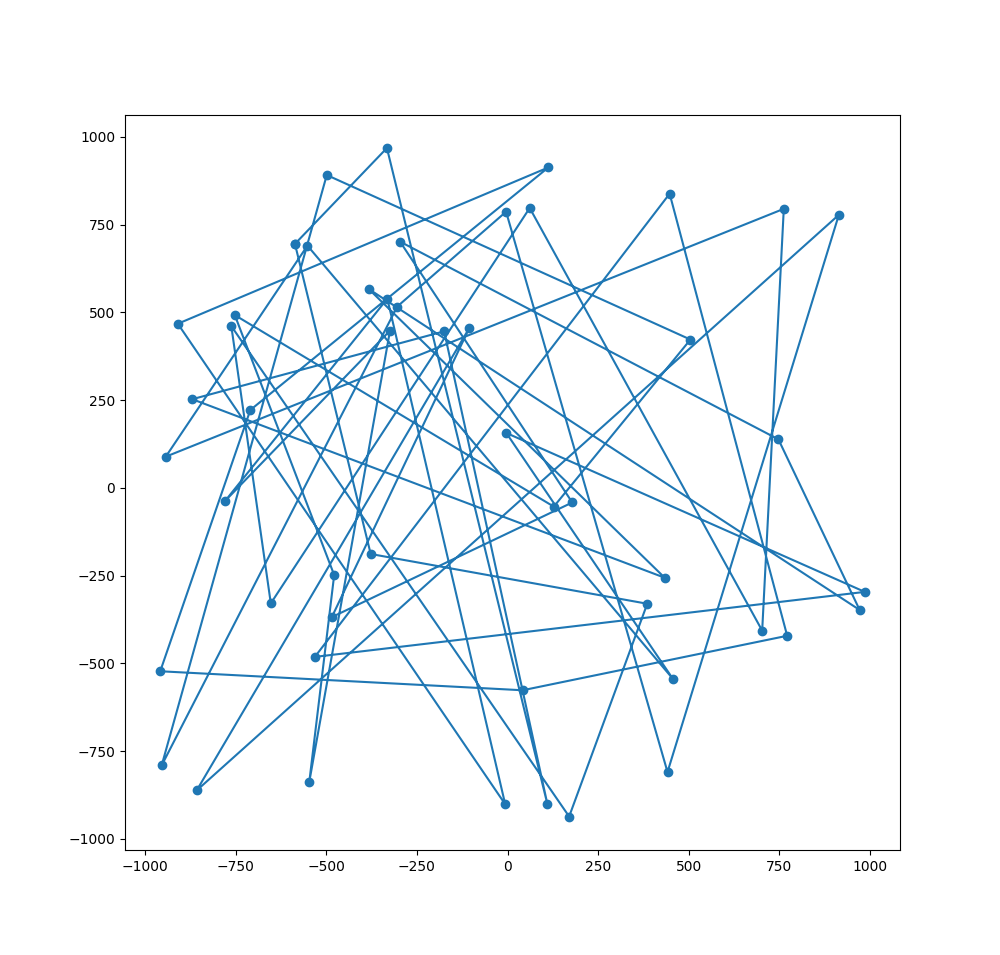
\includegraphics[width=6cm]{lab4/img/tsp_n100_t20_uni_pre.png}}
            \subfloat[]{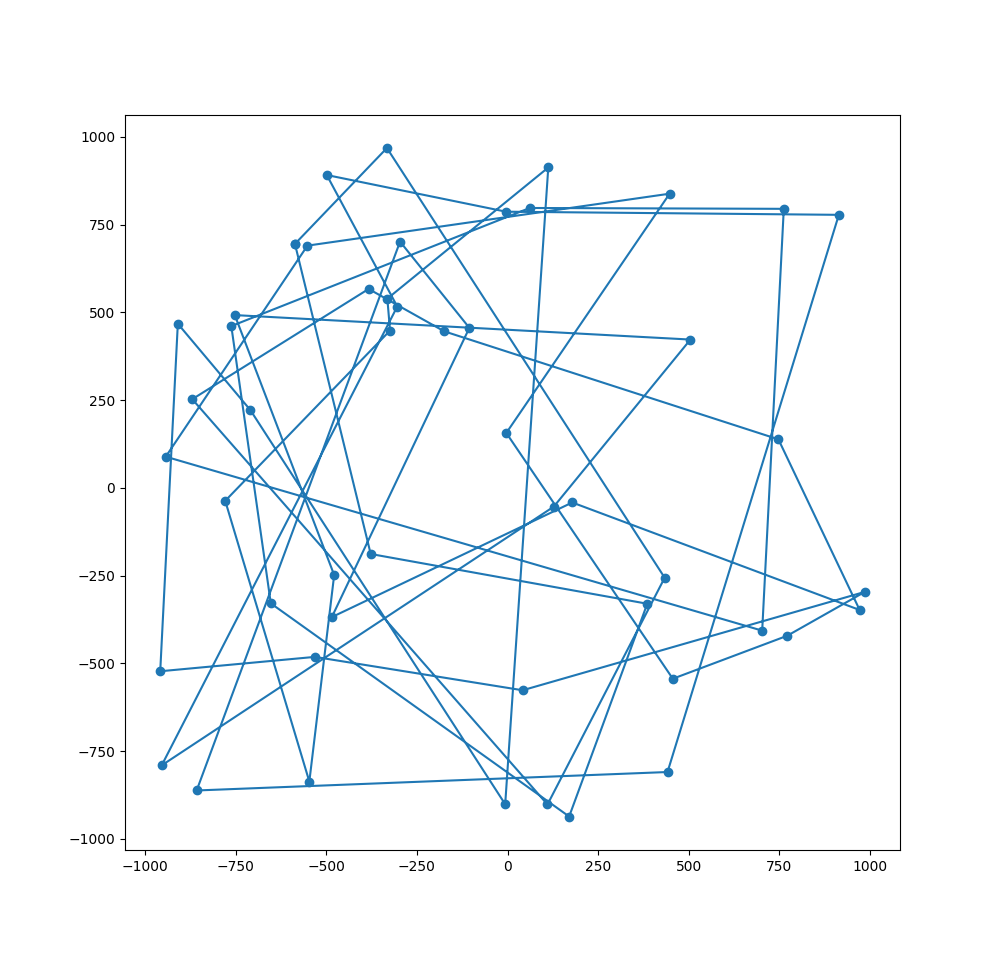
\includegraphics[width=6cm]{lab4/img/tsp_n100_t20_uni_post.png}}
            \subfloat[]{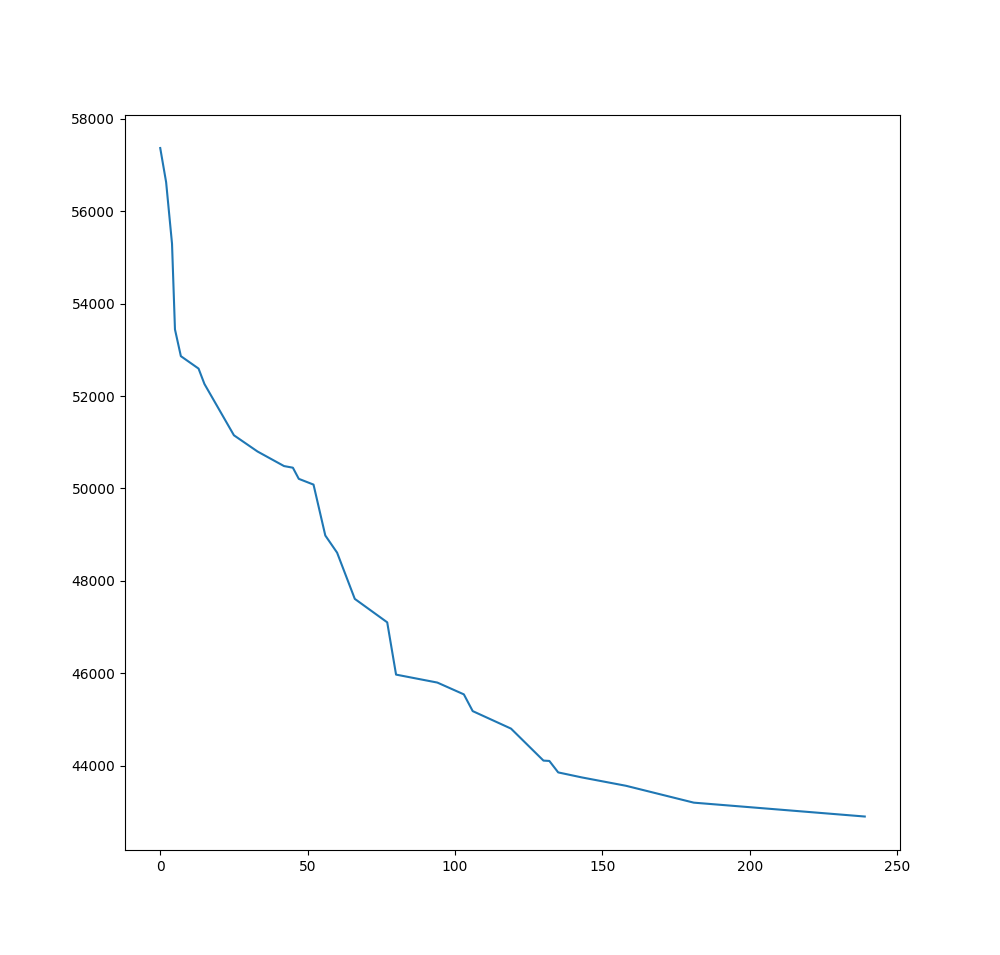
\includegraphics[width=6cm]{lab4/img/tsp_n100_t20_uni_plot.png}}
            \caption{Rozkład jednostajny, $100$ punktów, temperatura $20$, optymalizacja trasy $25.52\%$}
        \end{figure}\\
        \begin{figure}[h!]
            \centering
            \subfloat[]{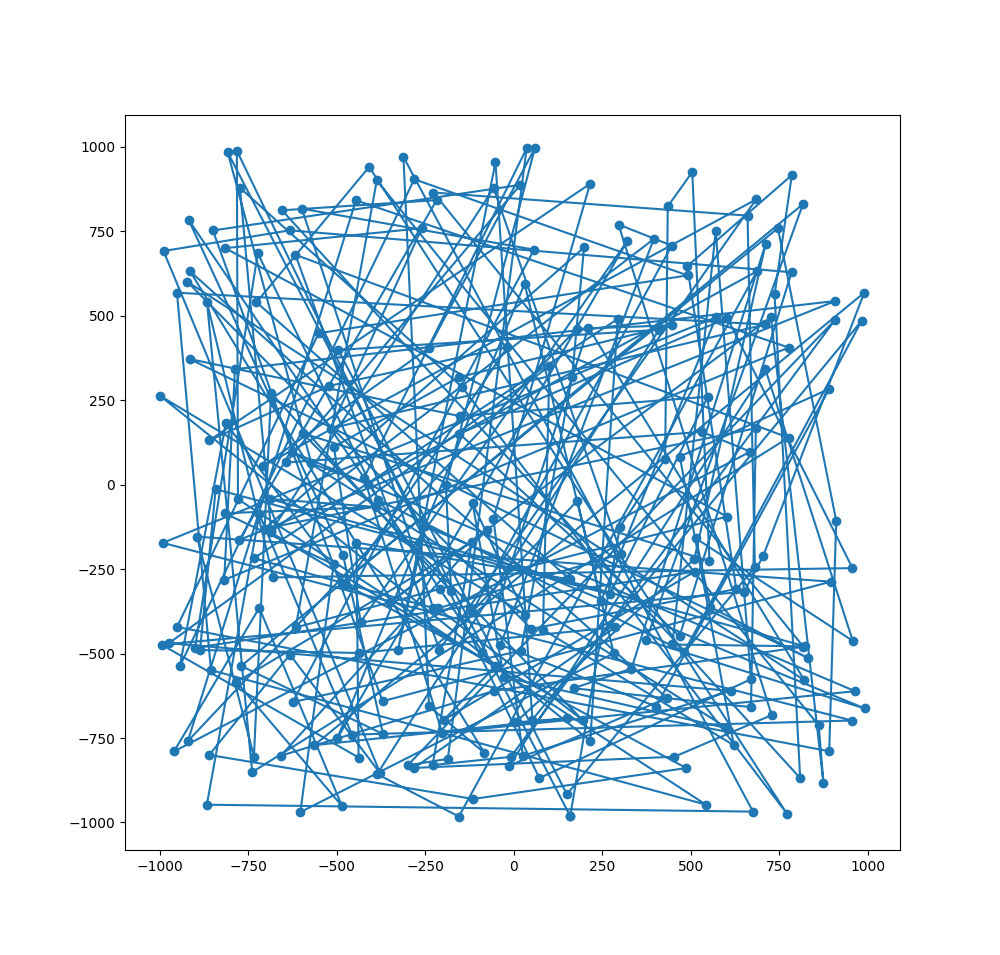
\includegraphics[width=6cm]{lab4/img/tsp_n500_t20_uni_pre.png}}
            \subfloat[]{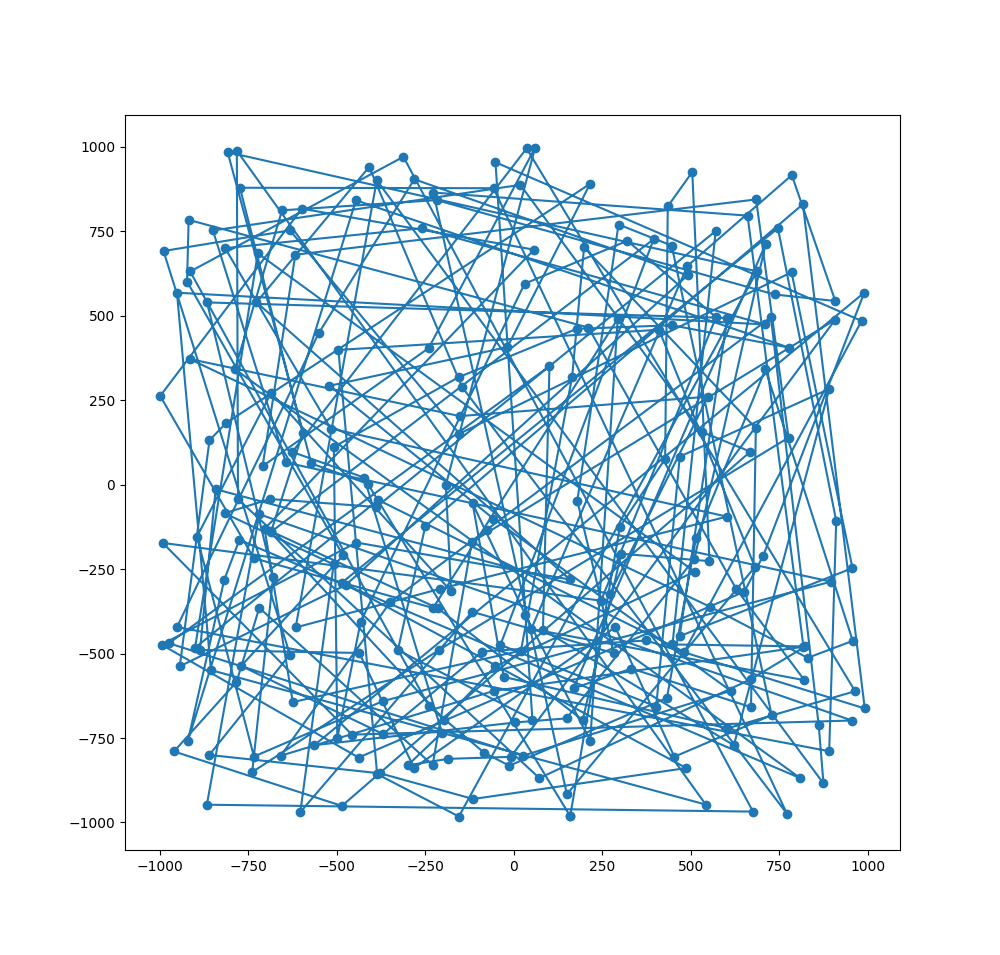
\includegraphics[width=6cm]{lab4/img/tsp_n500_t20_uni_post.png}}
            \subfloat[]{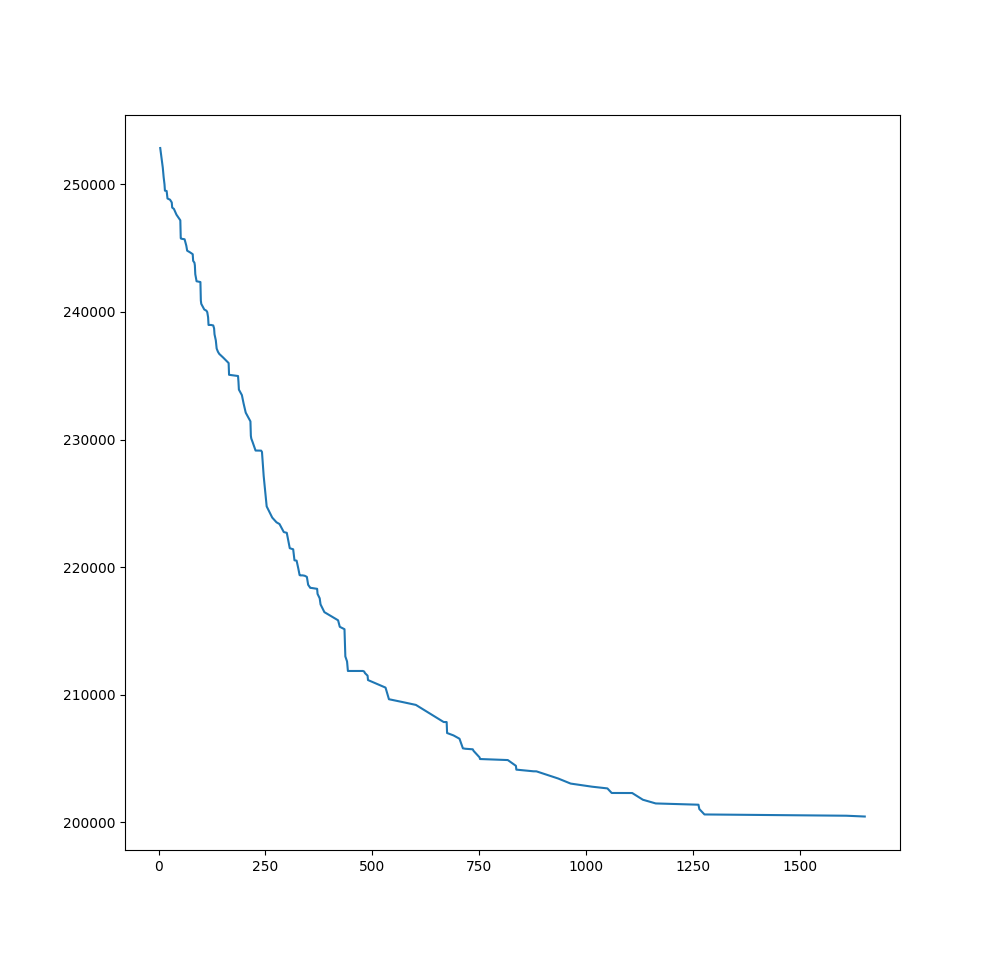
\includegraphics[width=6cm]{lab4/img/tsp_n500_t20_uni_plot.png}}
            \caption{Rozkład jednostajny, $500$ punktów, temperatura $20$, optymalizacja trasy $20.72\%$}
        \end{figure}\\
        \begin{figure}[h!]
            \centering
            \subfloat[]{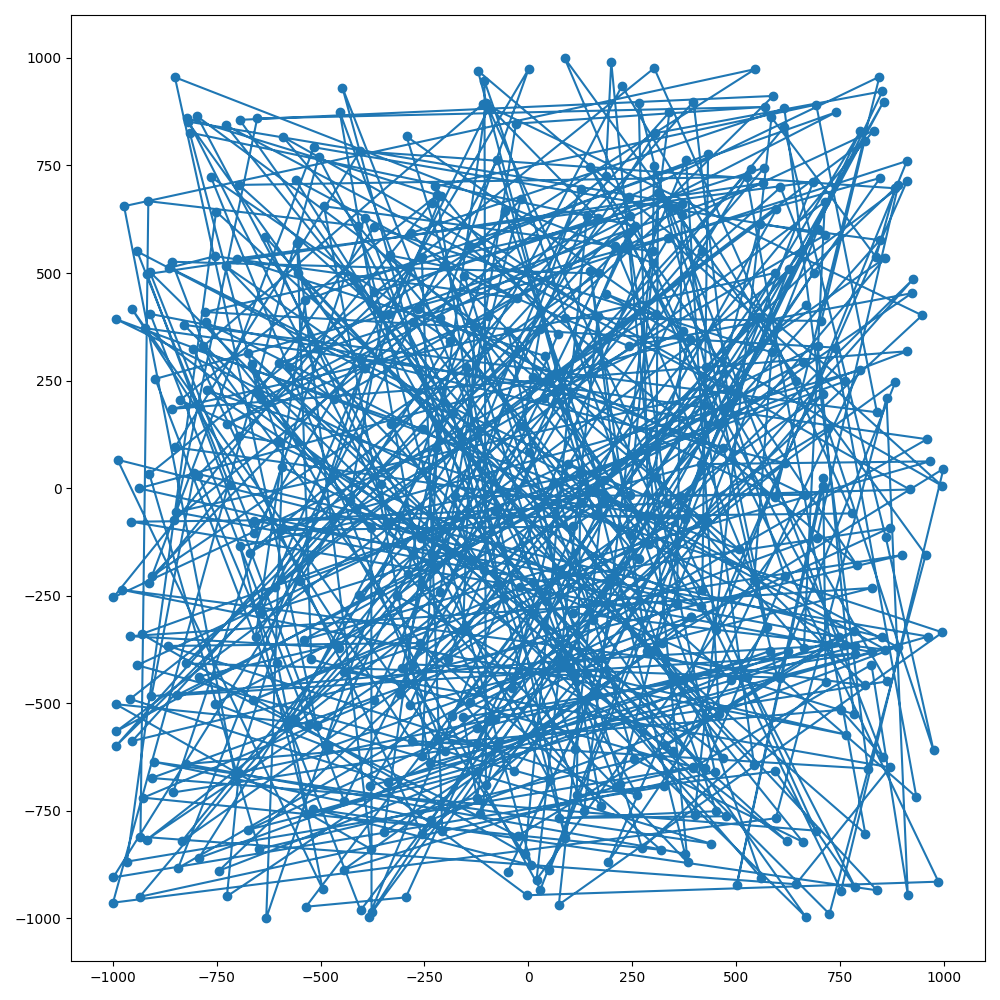
\includegraphics[width=6cm]{lab4/img/tsp_n1000_t31_uni_pre.png}}
            \subfloat[]{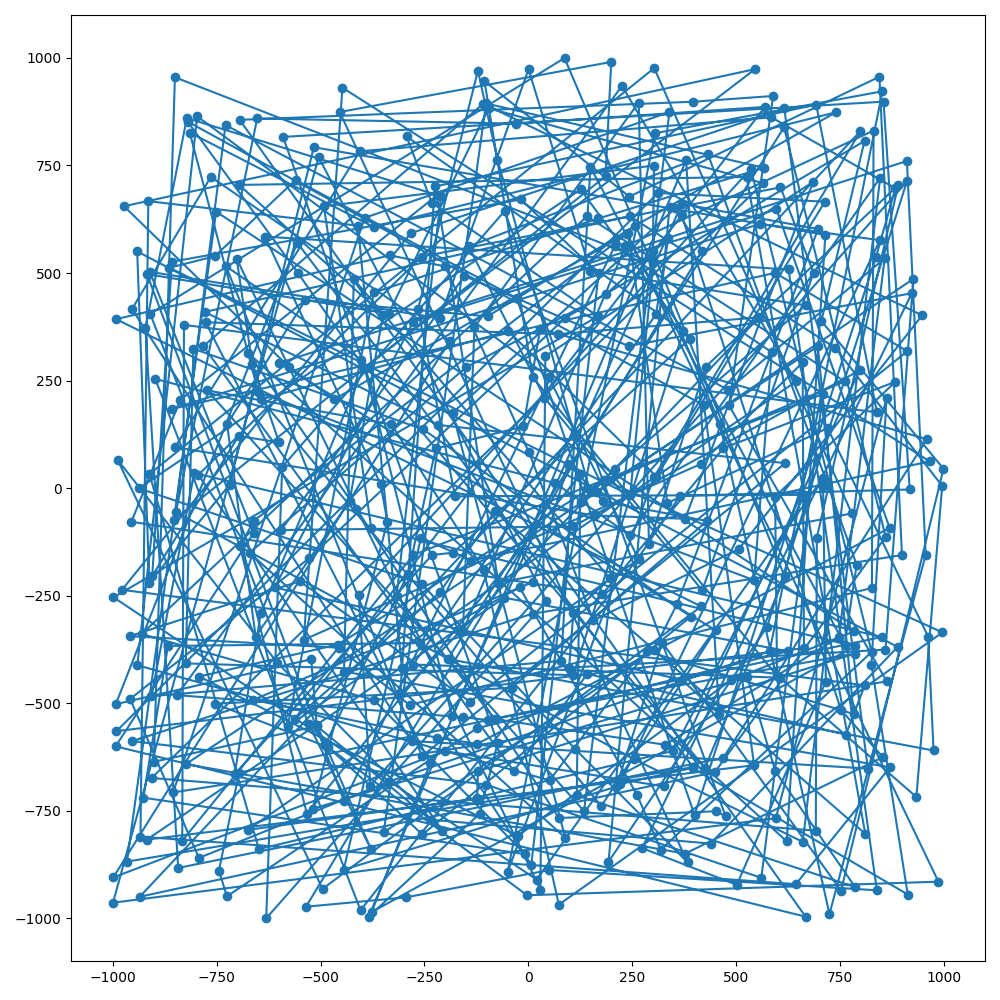
\includegraphics[width=6cm]{lab4/img/tsp_n1000_t31_uni_post.png}}
            \subfloat[]{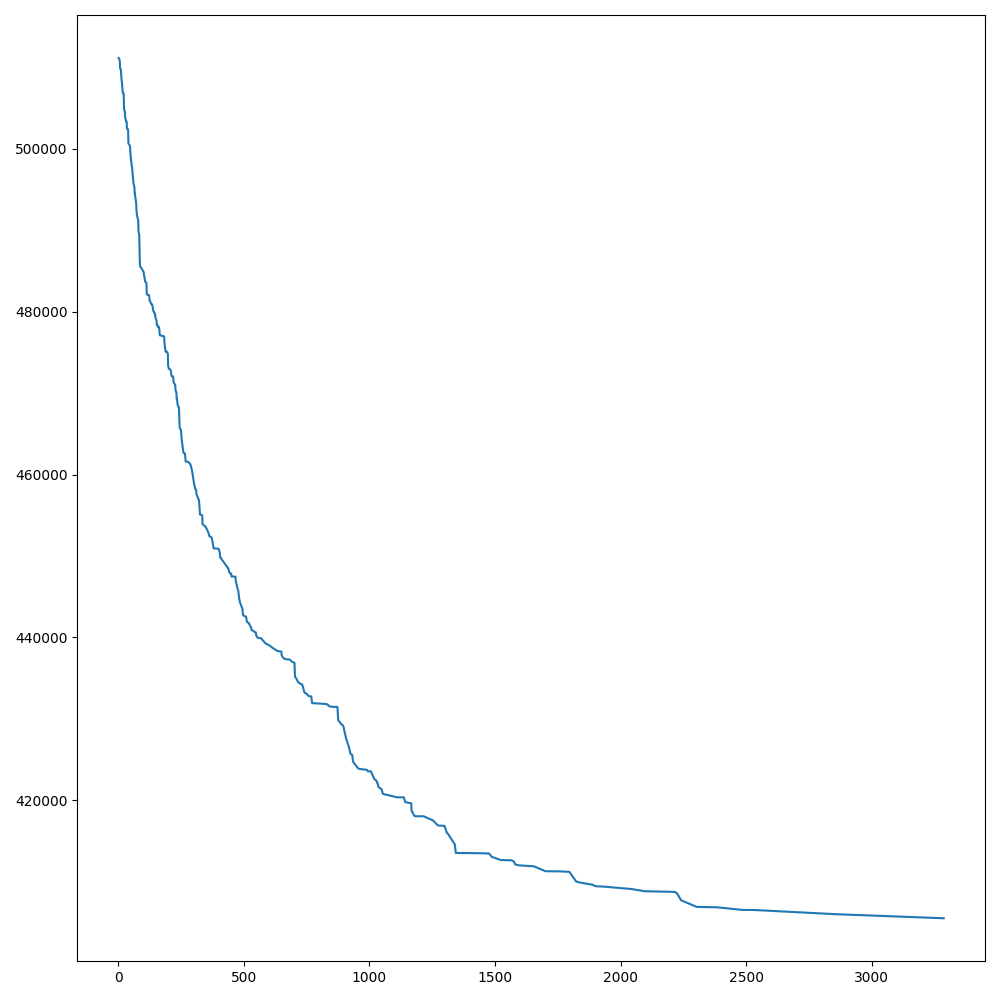
\includegraphics[width=6cm]{lab4/img/tsp_n1000_t31_uni_plot.png}}
            \caption{Rozkład jednostajny, $1000$ punktów, temperatura $31$, optymalizacja trasy $20.69\%$}
        \end{figure}\\
        \begin{figure}[h!]
            \centering
            \subfloat[]{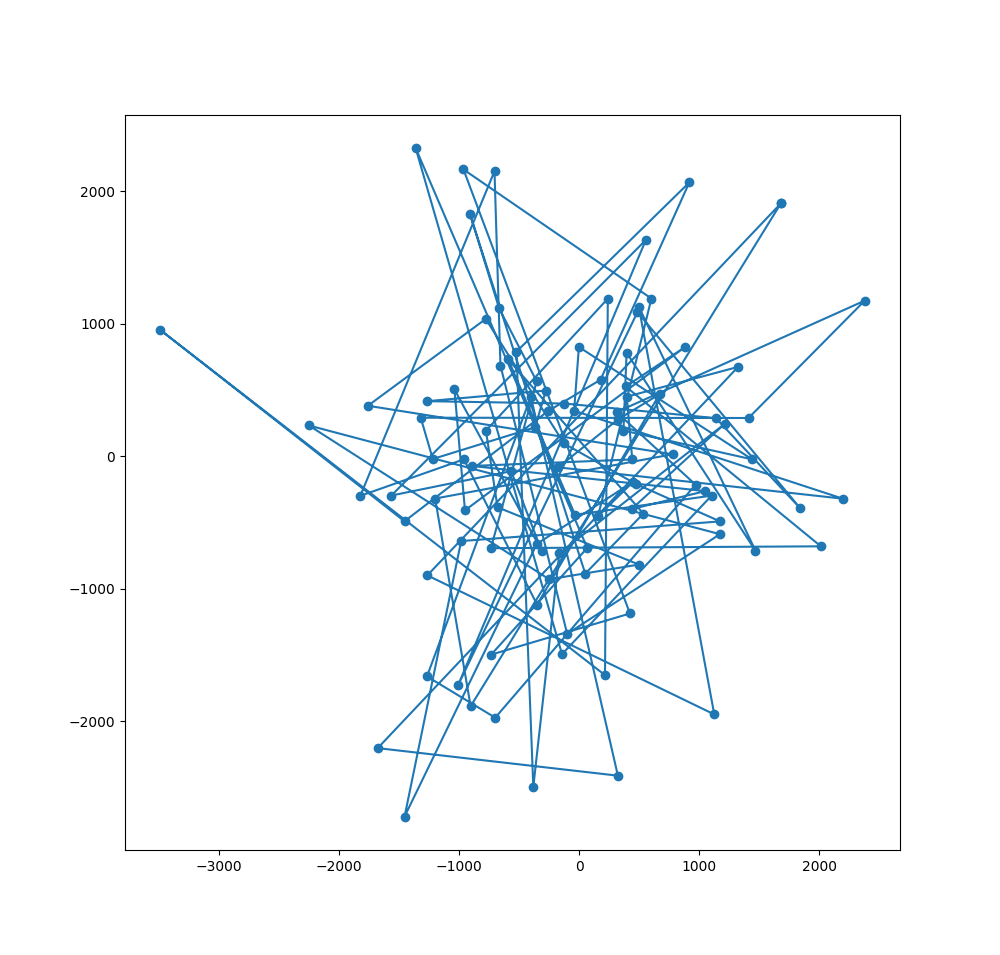
\includegraphics[width=6cm]{lab4/img/tsp_n100_t20_norm_0.png}}
            \subfloat[]{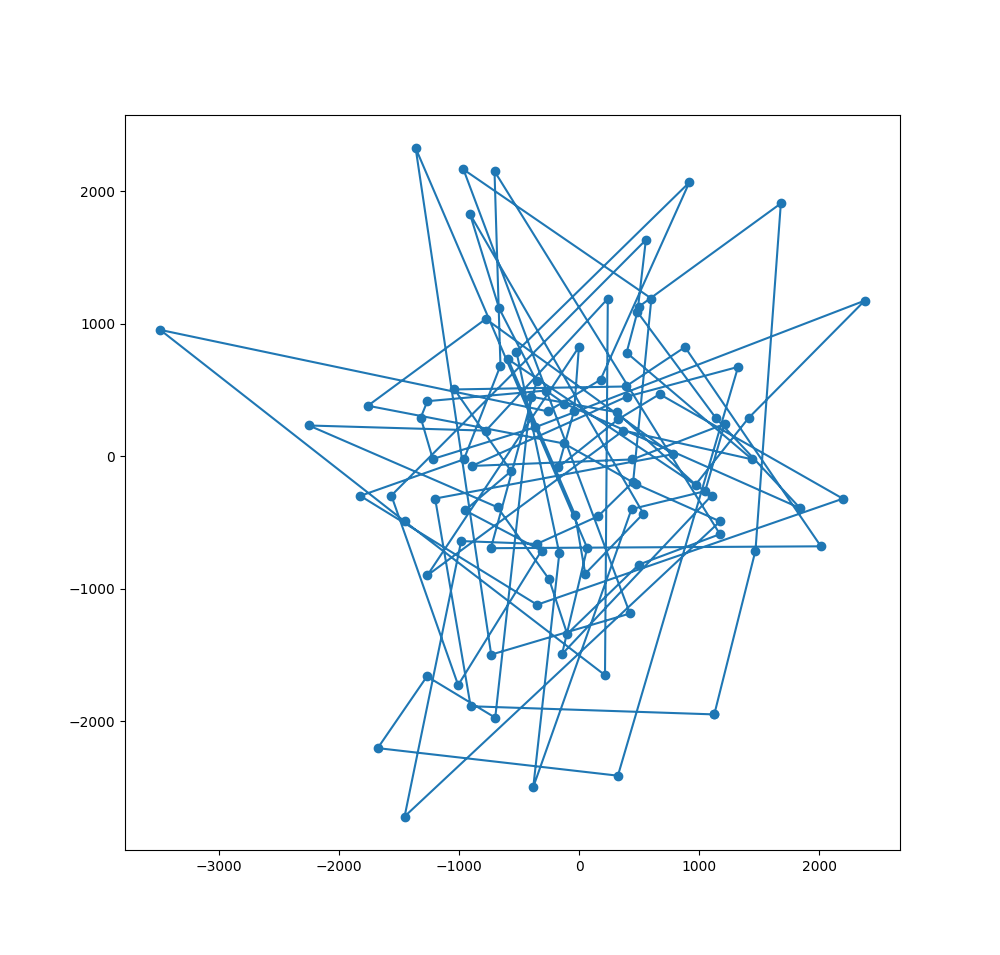
\includegraphics[width=6cm]{lab4/img/tsp_n100_t20_norm_1.png}}
            \subfloat[]{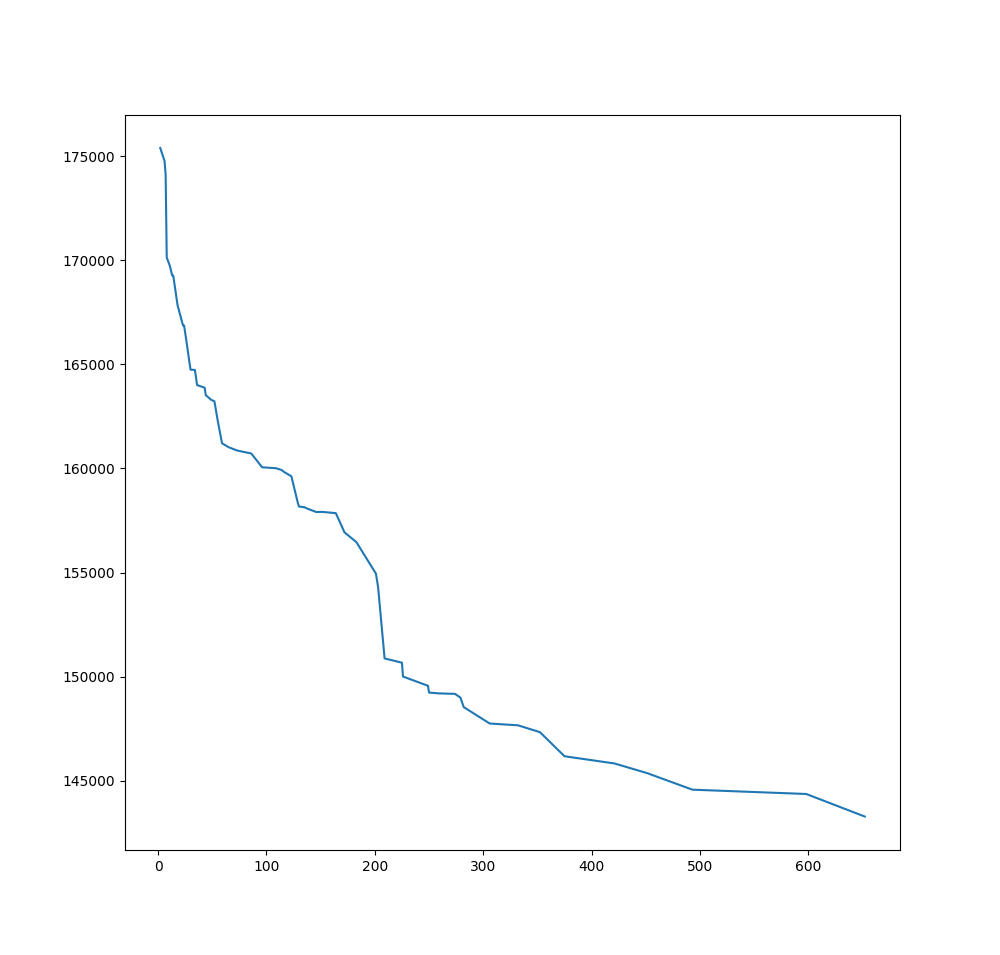
\includegraphics[width=6cm]{lab4/img/tsp_n100_t20_norm_2.png}}
            \caption{Rozkład normalny, $100$ punktów, temperatura $20$, optymalizacja trasy $18.38\%$}
        \end{figure}\\
        \begin{figure}[h!]
            \centering
            \subfloat[]{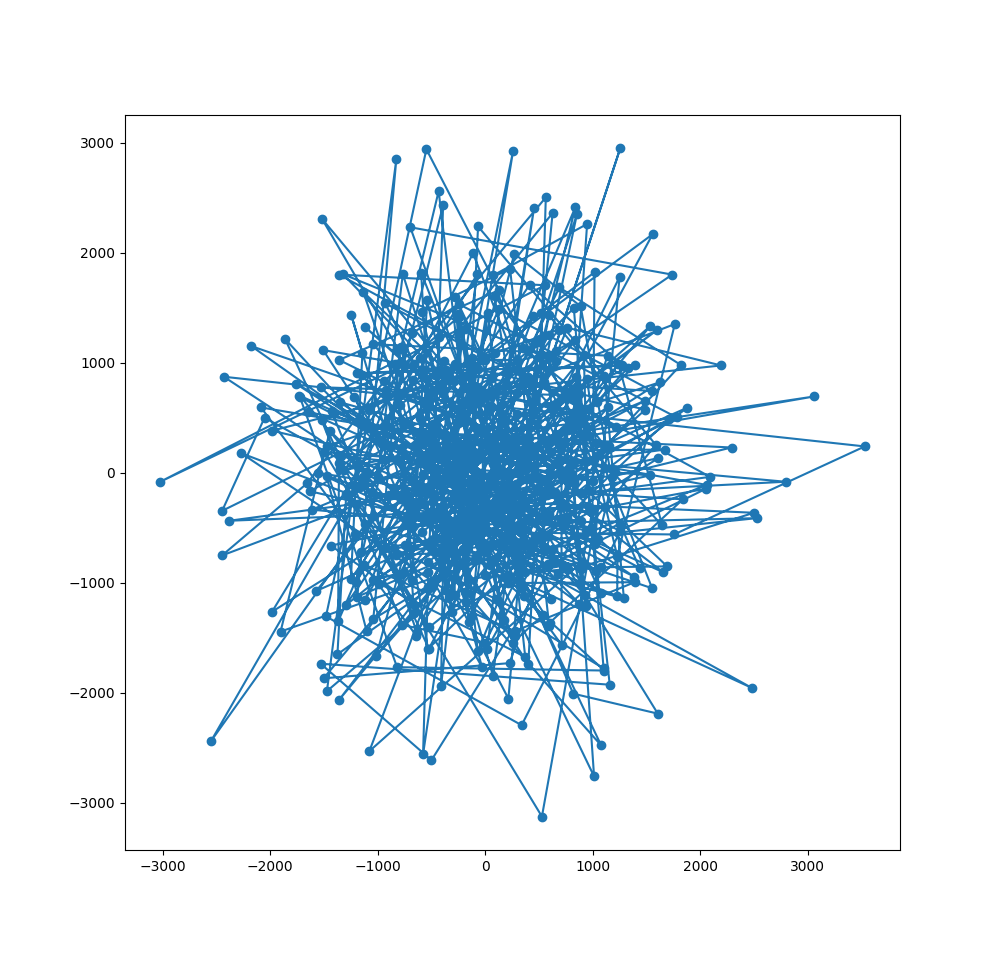
\includegraphics[width=6cm]{lab4/img/tsp_n500_t20_norm_0.png}}
            \subfloat[]{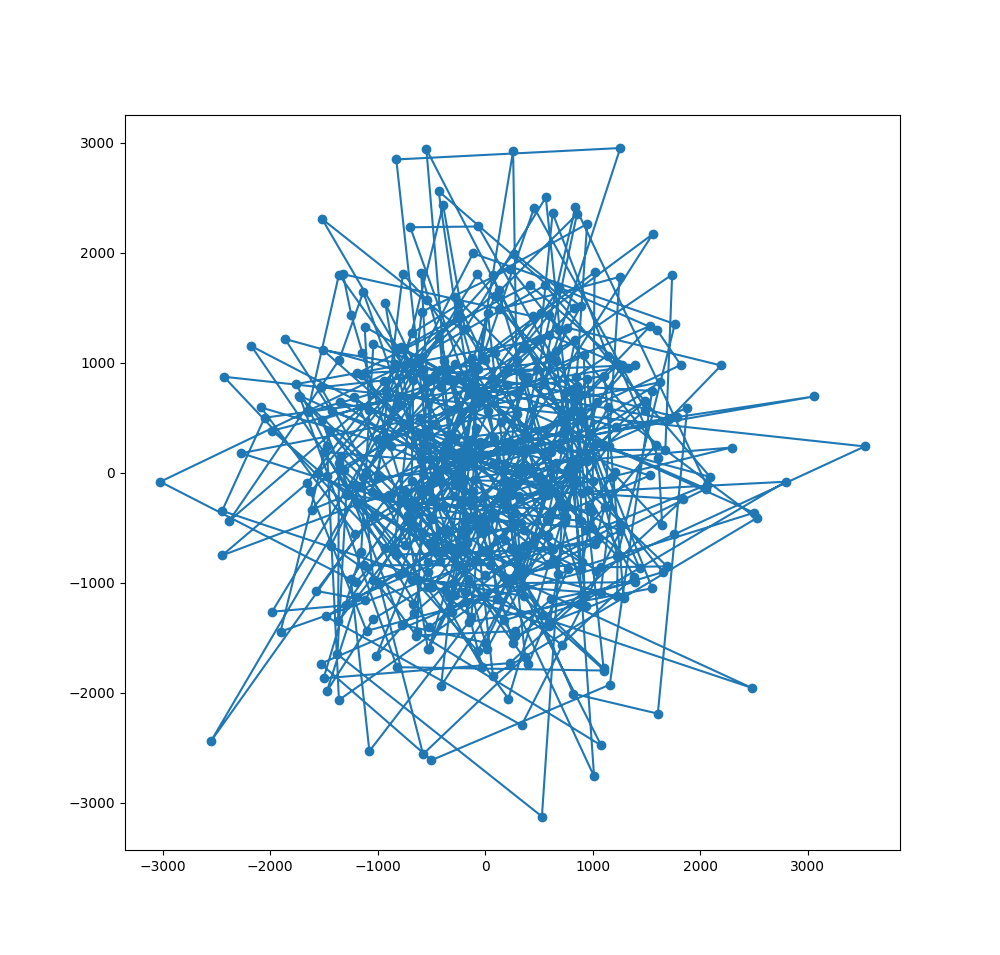
\includegraphics[width=6cm]{lab4/img/tsp_n500_t20_norm_1.png}}
            \subfloat[]{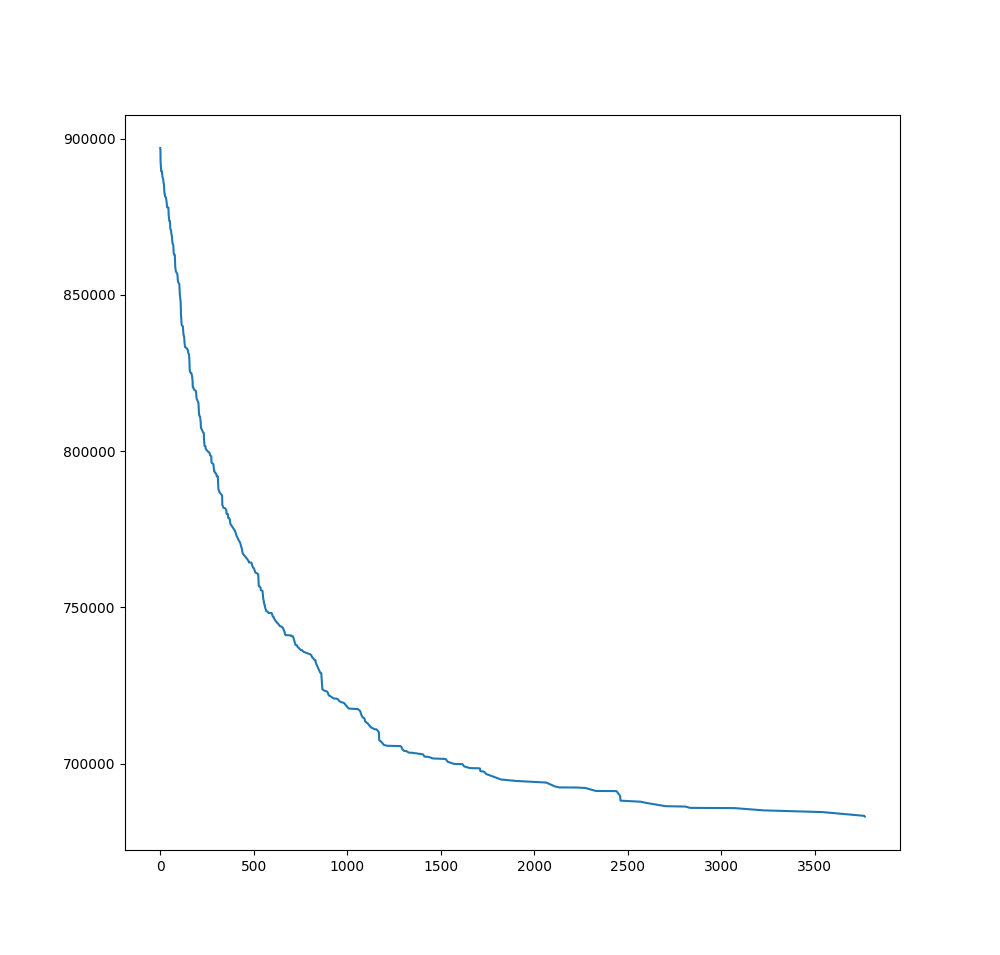
\includegraphics[width=6cm]{lab4/img/tsp_n500_t20_norm_2.png}}
            \caption{Rozkład normalny, $500$ punktów, temperatura $20$, optymalizacja trasy $24.2\%$}
        \end{figure}\\
        \begin{figure}[h!]
            \centering
            \subfloat[]{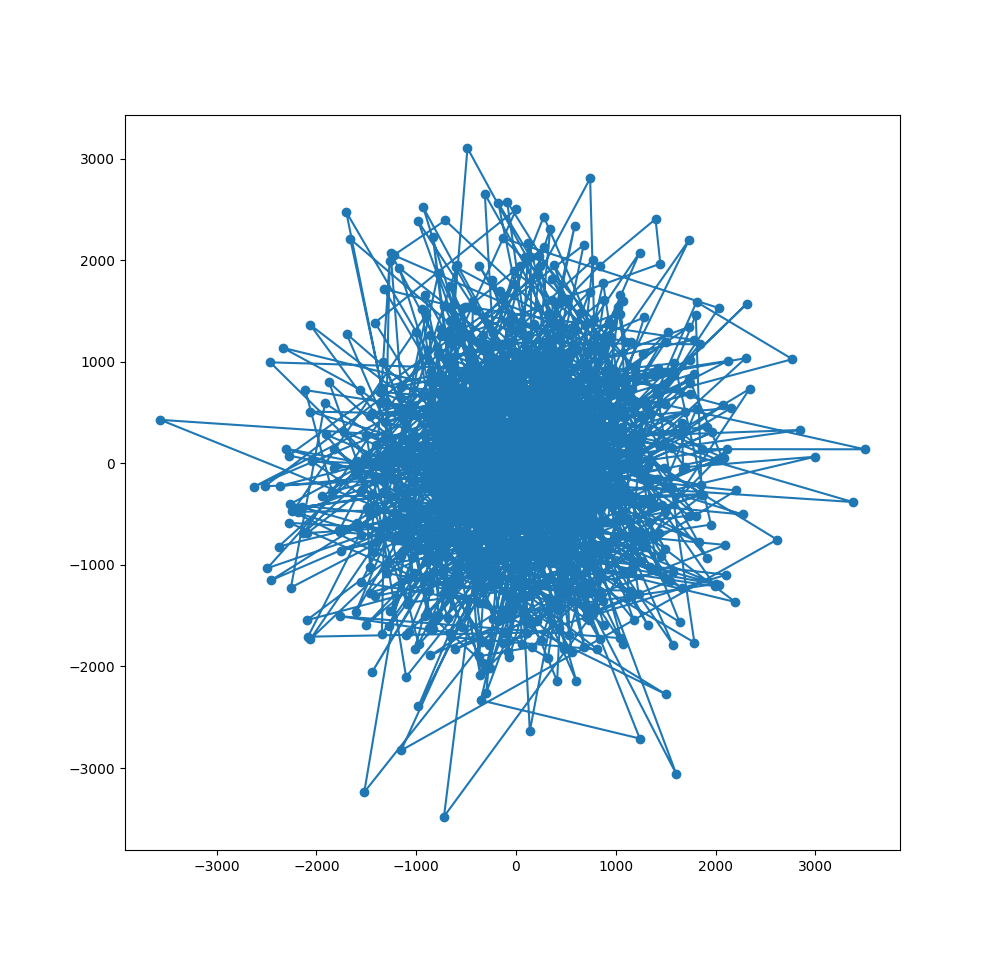
\includegraphics[width=6cm]{lab4/img/tsp_n1000_t31_norm_0.png}}
            \subfloat[]{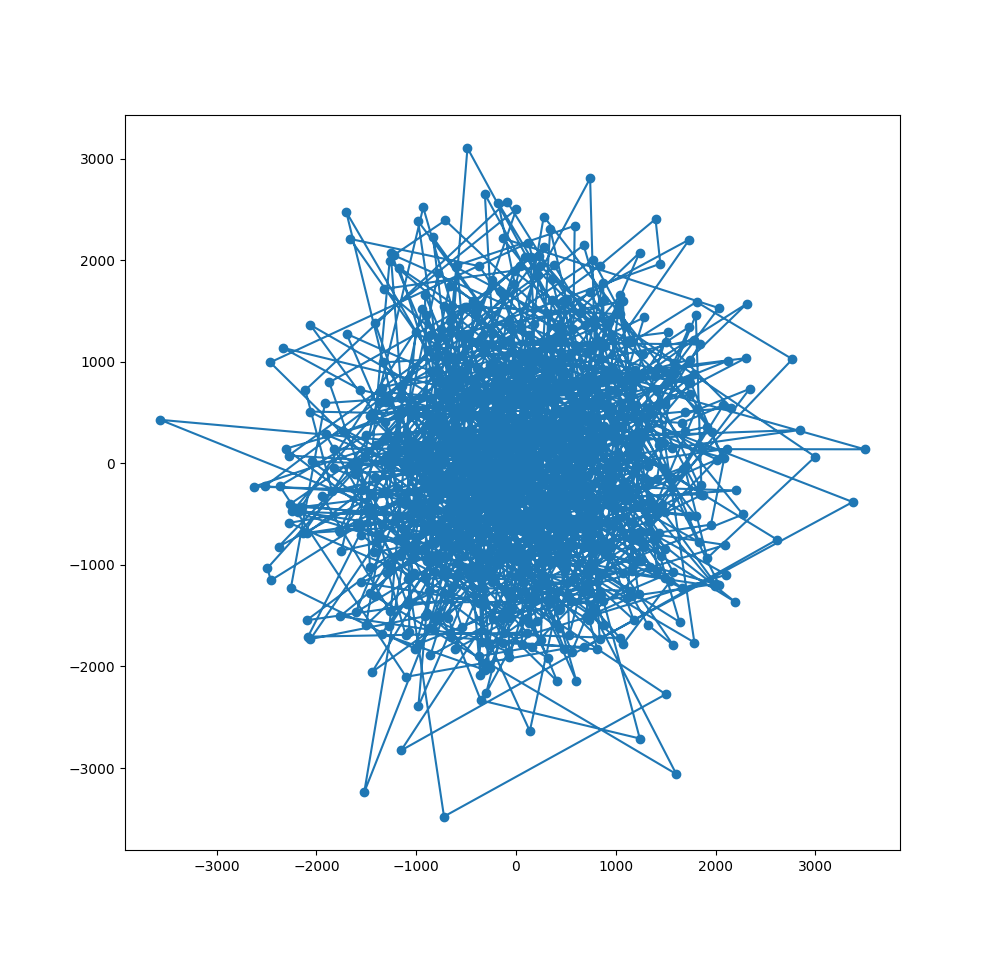
\includegraphics[width=6cm]{lab4/img/tsp_n1000_t31_norm_1.png}}
            \subfloat[]{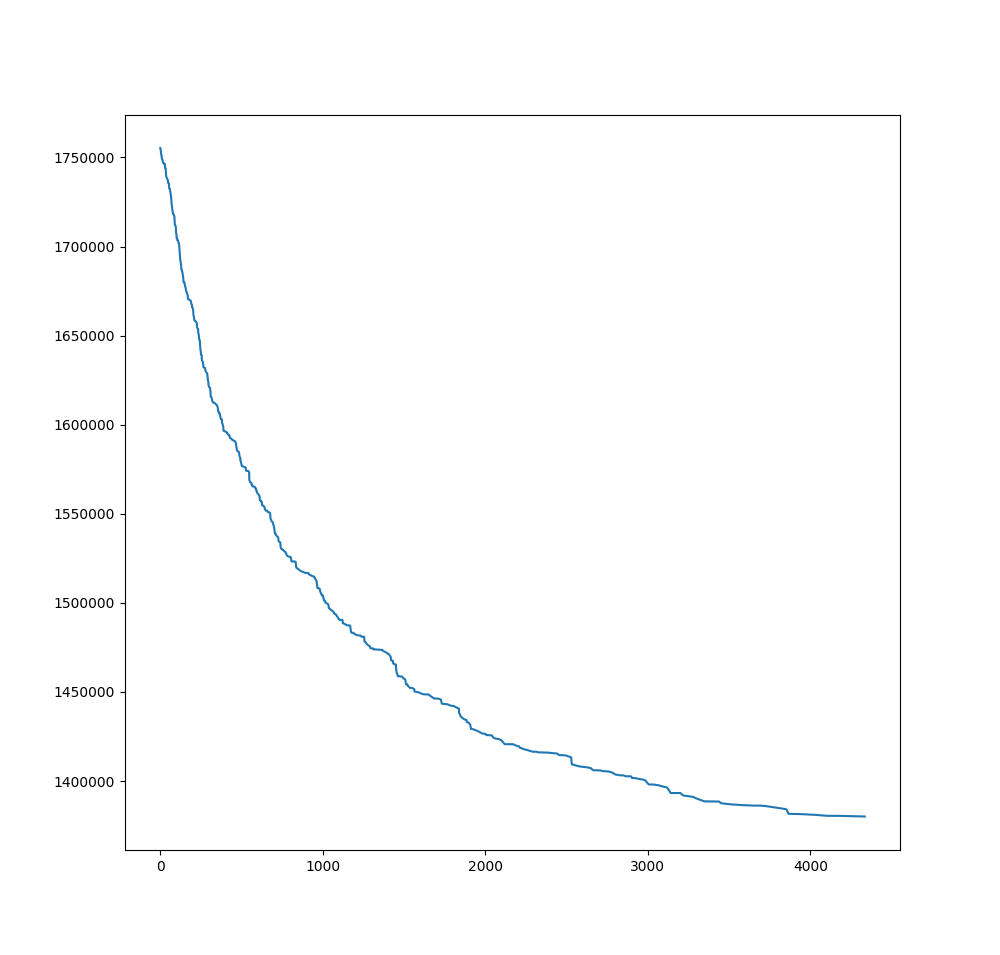
\includegraphics[width=6cm]{lab4/img/tsp_n1000_t31_norm_2.png}}
            \caption{Rozkład normalny, $1000$ punktów, temperatura $31$, optymalizacja trasy $21.41\%$}
        \end{figure}\\
        \begin{figure}[h!]
            \centering
            \subfloat[]{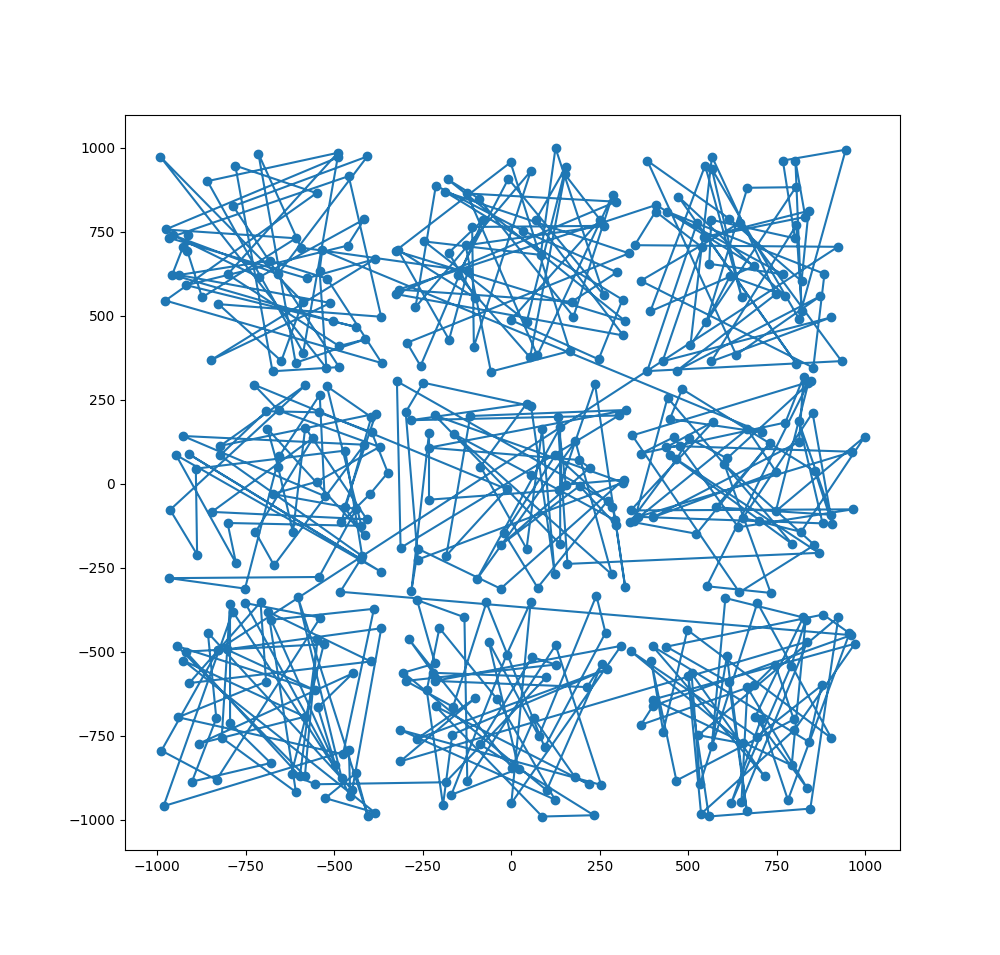
\includegraphics[width=6cm]{lab4/img/tsp_n100_t20_grp_0.png}}
            \subfloat[]{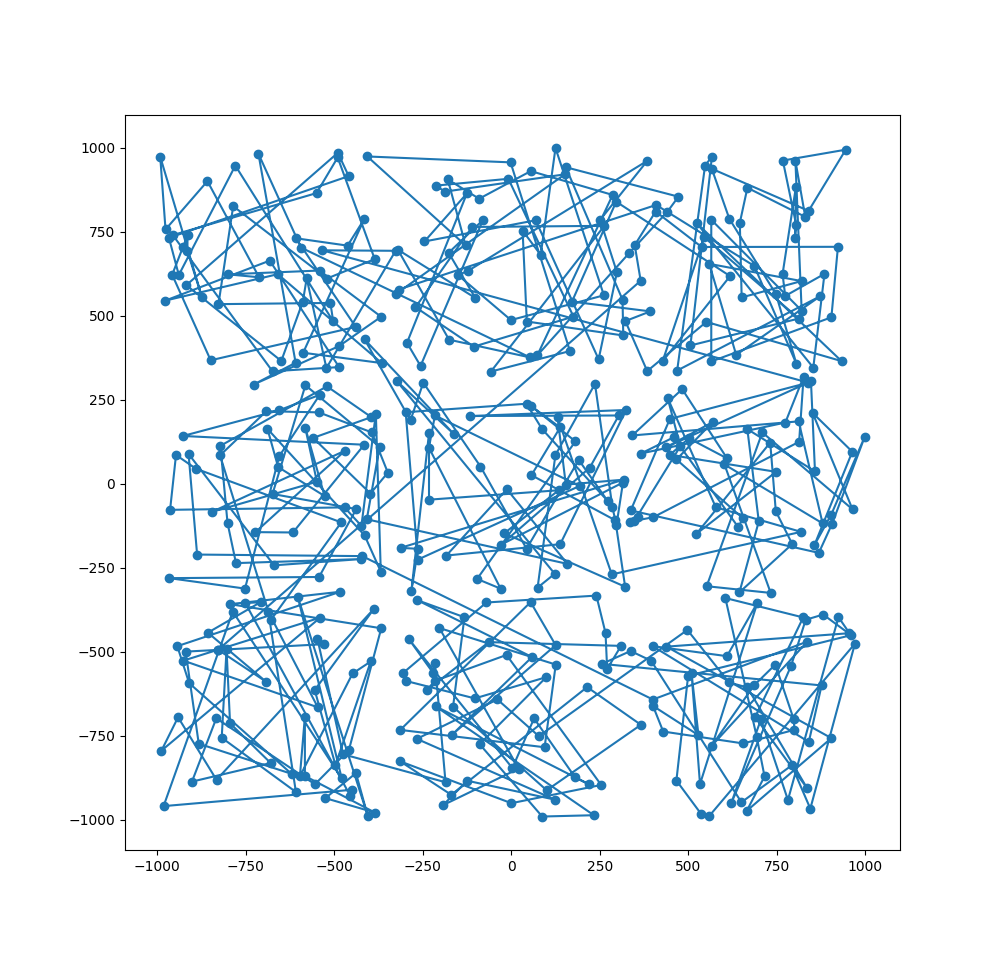
\includegraphics[width=6cm]{lab4/img/tsp_n100_t20_grp_1.png}}
            \subfloat[]{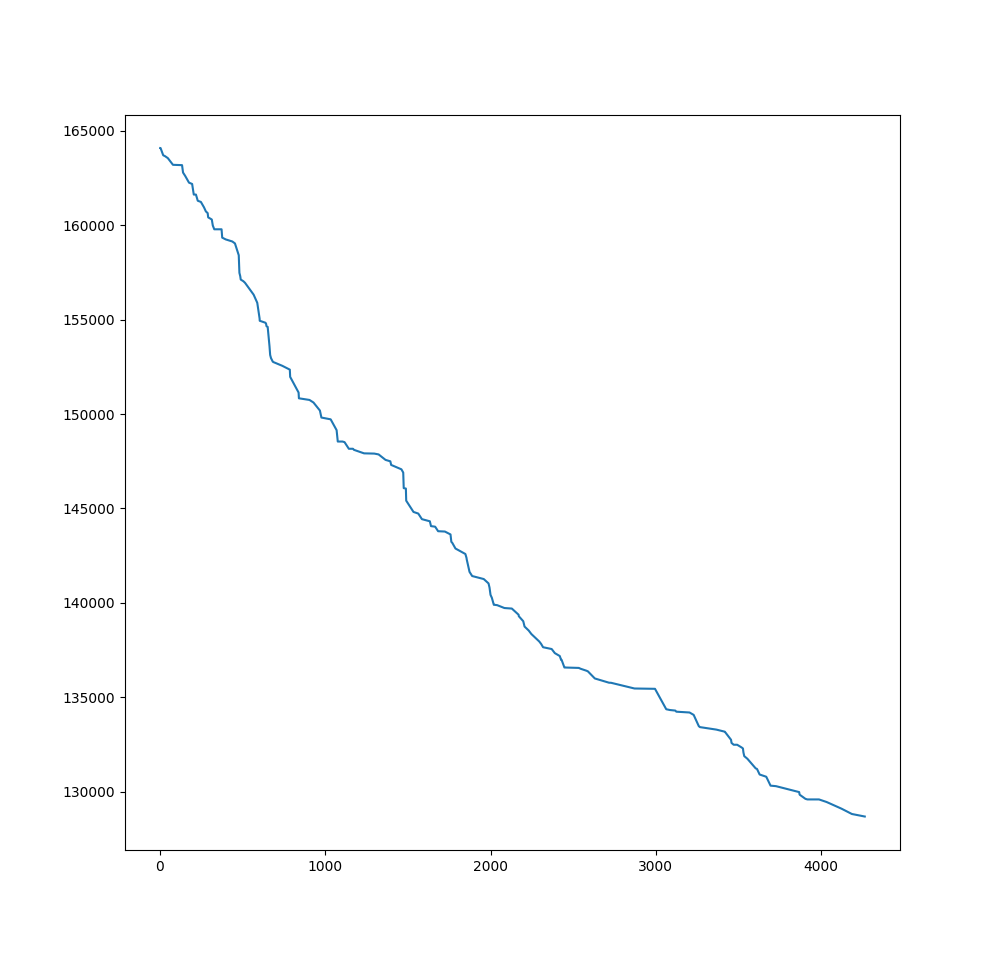
\includegraphics[width=6cm]{lab4/img/tsp_n100_t20_grp_2.png}}
            \caption{Rozkład grupowy, $100$ punktów, temperatura $20$, optymalizacja trasy $21.87\%$}
        \end{figure}\\
        \begin{figure}[h!]
            \centering
            \subfloat[]{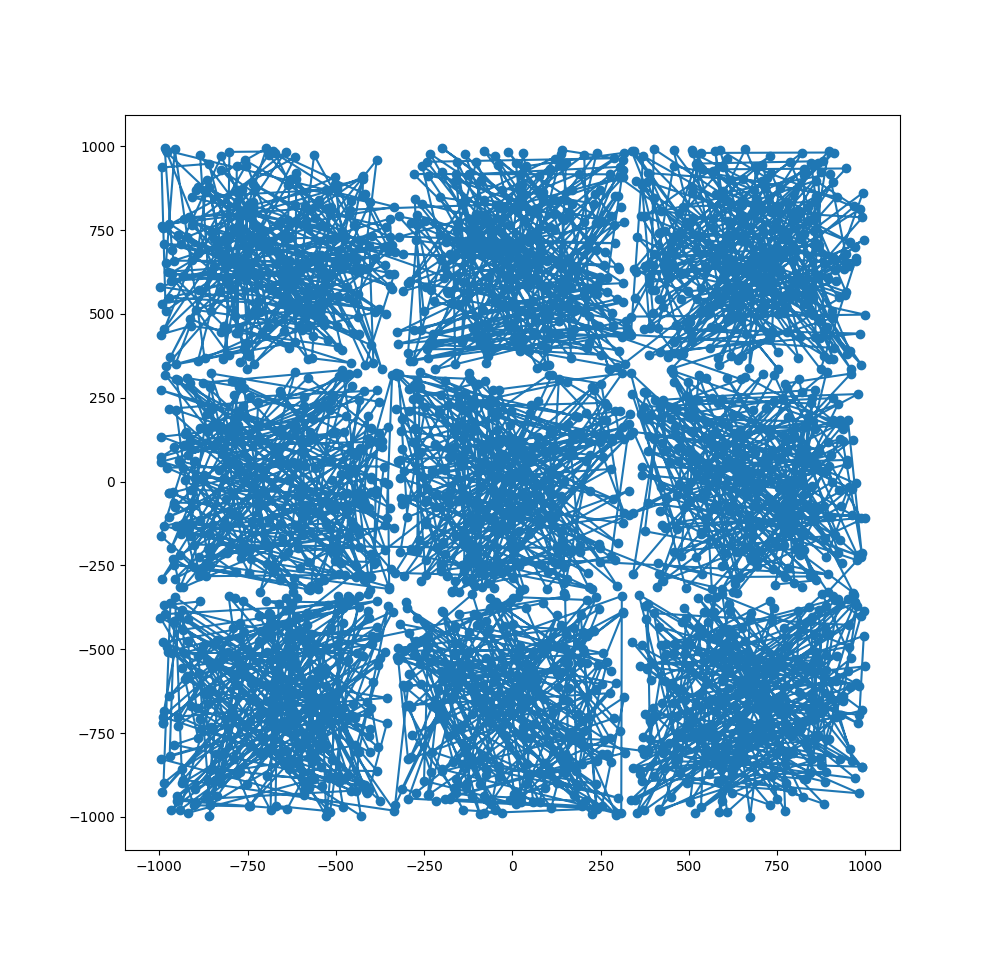
\includegraphics[width=6cm]{lab4/img/tsp_n500_t20_grp_0.png}}
            \subfloat[]{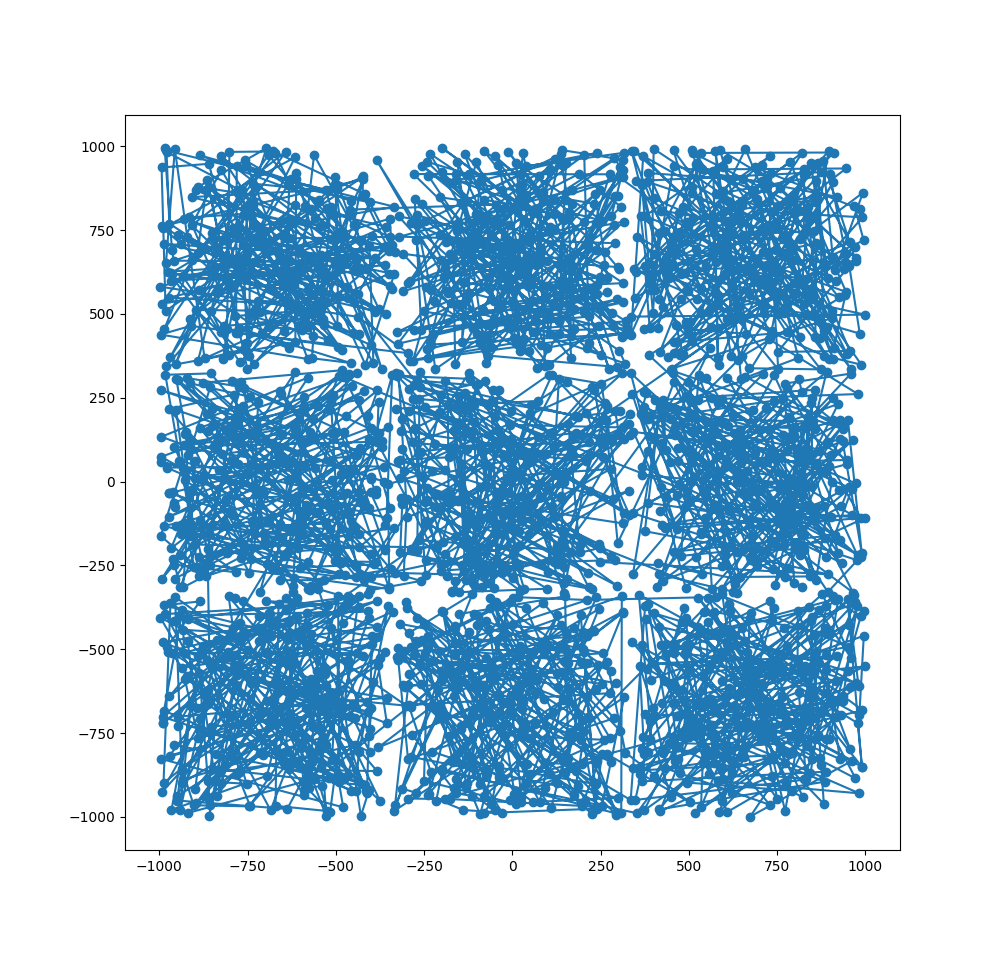
\includegraphics[width=6cm]{lab4/img/tsp_n500_t20_grp_1.png}}
            \subfloat[]{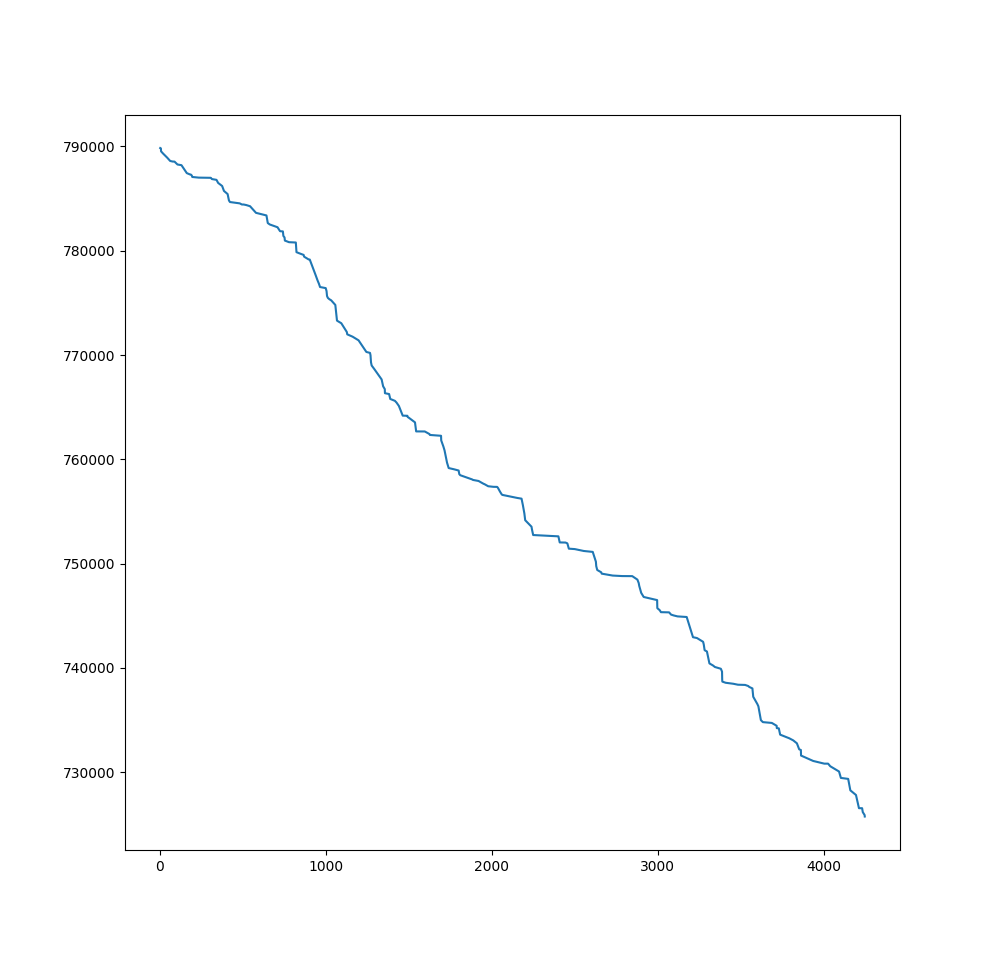
\includegraphics[width=6cm]{lab4/img/tsp_n500_t20_grp_2.png}}
            \caption{Rozkład grupowy, $500$ punktów, temperatura $20$, optymalizacja trasy $8.14\%$}
        \end{figure}\\
        \newpage
        \begin{figure}[h!]
            \centering
            \subfloat[]{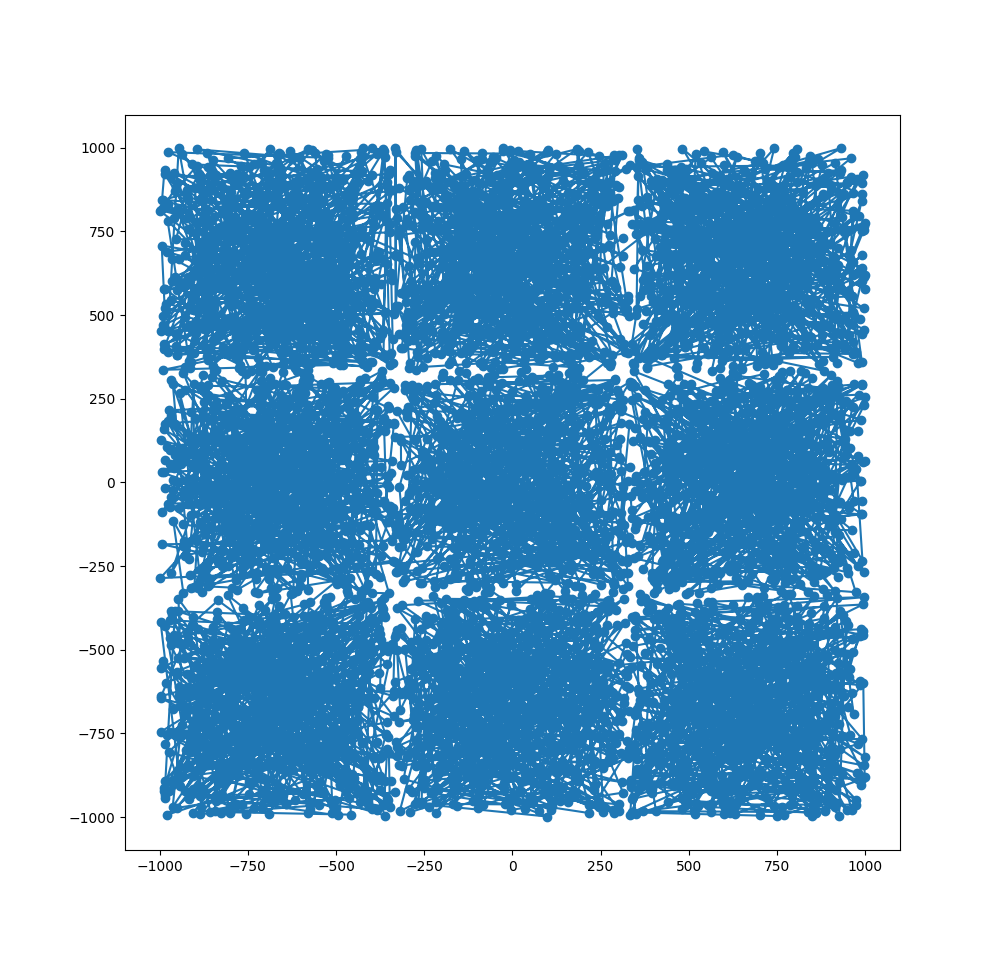
\includegraphics[width=6cm]{lab4/img/tsp_n1000_t31_grp_0.png}}
            \subfloat[]{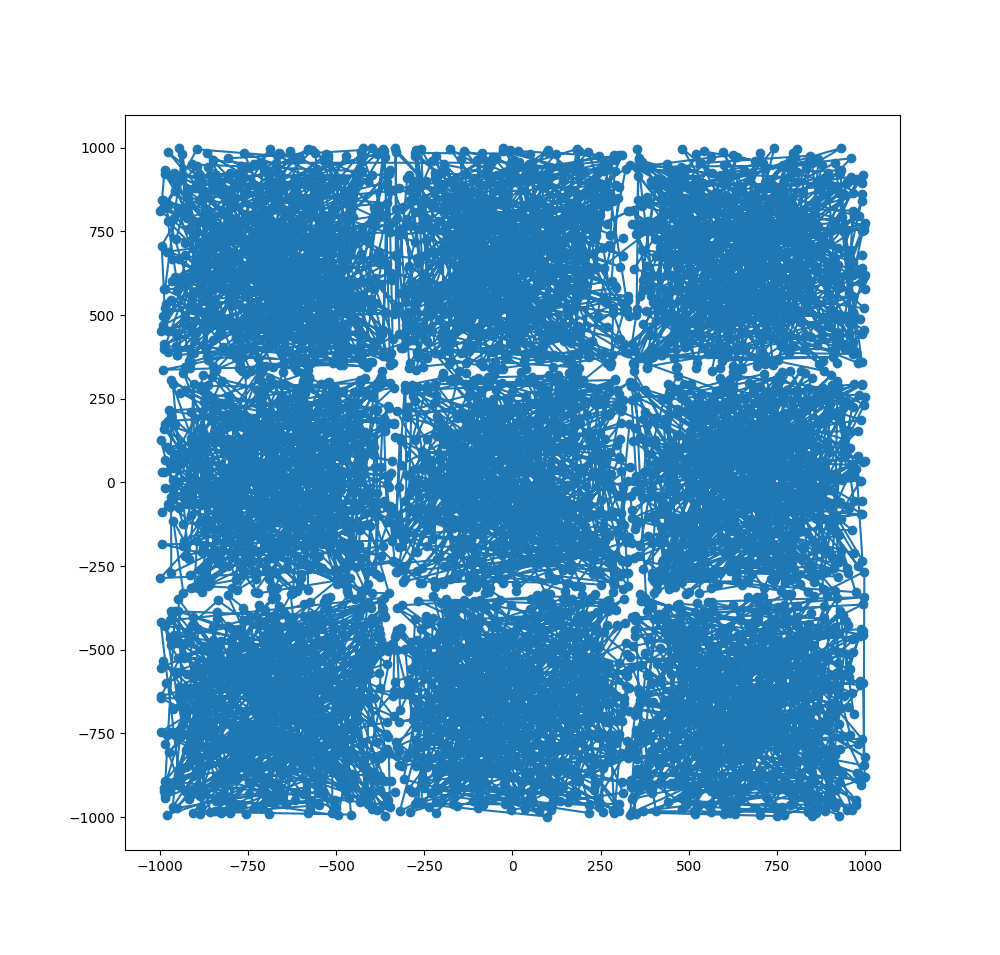
\includegraphics[width=6cm]{lab4/img/tsp_n1000_t31_grp_1.png}}
            \subfloat[]{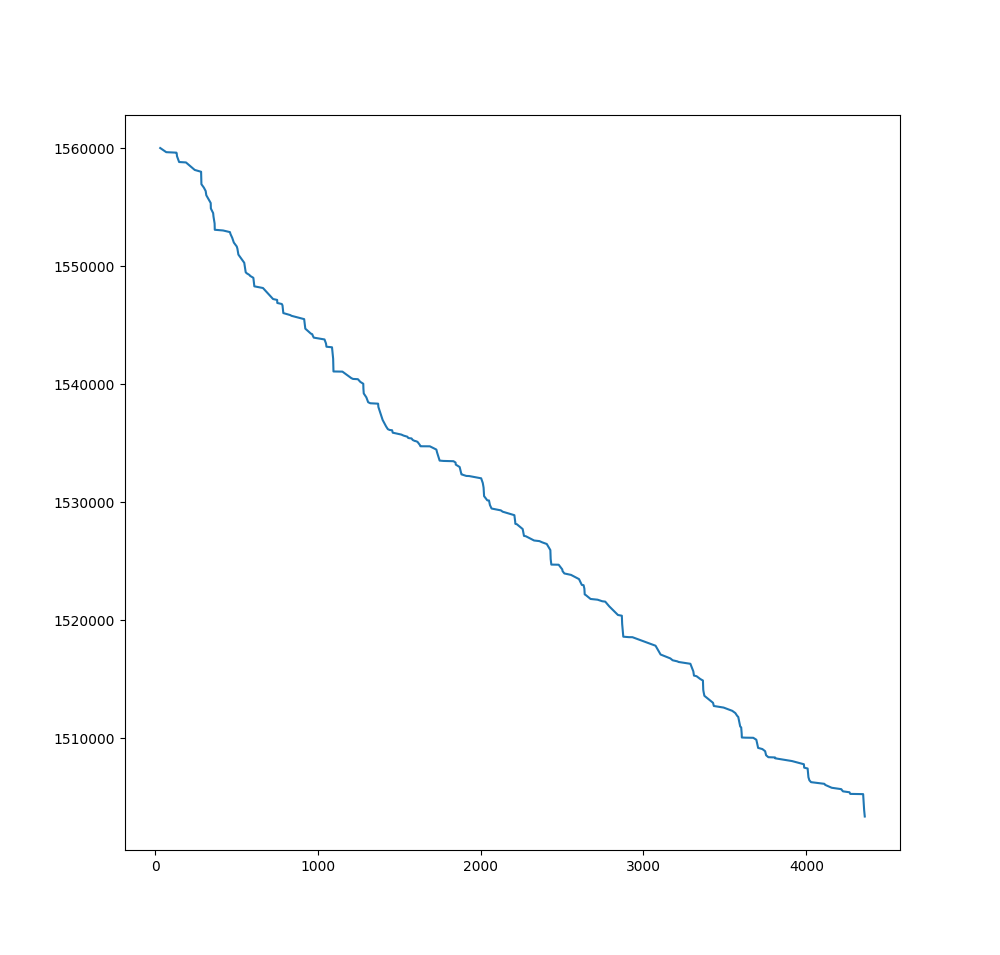
\includegraphics[width=6cm]{lab4/img/tsp_n1000_t31_grp_2.png}}
            \caption{Rozkład grupowy, $1000$ punktów, temperatura $31$, optymalizacja trasy $3.67\%$}
        \end{figure}\\
        % \newpage
        \FloatBarrier
        
        Następnie porównałem obliczoną minimalizację funkcji kosztu w zależności od sposobu generacji stanu sąsiedniego, otrzymując poniższe wyniki (\textit{Arbitrary} - funkcja zamieniająca dwa losowe indeksy, \textit{Consecutive} - funkcja zamieniająca dwa kolejne elementy, \textit{Reverse} - funkcja odwracająca losowy fragment). 
        \begin{center}
            \begin{table}[ht]
                \centering
                \begin{tabular}{|c|c|c|c|}
                    \hline
                    Dane & Arbitrary & Consecutive & Reverse \\
                    \specialrule{1pt}{1pt}{1pt}
                    Rozkład jednostajny, $N=100$ & $72.11\%$ & $26.45\%$& \cellcolor{green!40}$78.8\%$\\
                    \hline
                    Rozkład normalny, $N=100$ & $61.79\%$ & $17.72\%$& \cellcolor{green!40}$71.34\%$\\
                    \hline 
                    Rozkład grupowy, $N=100$ & \cellcolor{green!40}$22.32\%$ & $20.51\%$& $21.36\%$\\
                    \hline
                    Rozkład jednostajny, $N=500$ & $51.06\%$ & $25.2\%$&\cellcolor{green!40} $60.31\%$\\
                    \hline 
                    Rozkład normalny, $N=500$ & $47.79\%$ & $21.84\%$&\cellcolor{green!40} $53.97\%$\\
                    \hline 
                    Rozkład grupowy, $N=500$ & $7.81\%$ & \cellcolor{green!40}$18.91\%$& $5.61\%$\\
                    \hline 
                    Rozkład jednostajny, $N=1000$ & $44.28\%$ & $22.61\%$&\cellcolor{green!40} $48.16\%$\\
                    \hline 
                    Rozkład normalny, $N=1000$ & $38.59\%$ & $19.67\%$&\cellcolor{green!40} $43.43\%$\\
                    \hline 
                    Rozkład grupowy, $N=1000$ & $4.92\%$ & \cellcolor{green!40}$14.8\%$& $3.5\%$\\
                    \hline 
                \end{tabular}
                \caption{Porównanie efektywności działania funkcji.}
                \label{tab:my_label}
            \end{table}
        \end{center}\\
        
        % \FloatBarrier
        Następnie przygotowałem funkcję obliczającą zachłanne przybliżenie problemu komiwojażera stosującą heurystykę najbliższego kroku. Dla tak zainicjalizowanych danych, z użyciem funkcji arbitrary swap, przeprowadziłem próbę skuteczności zaimplementowanego algorytmu wyżarzania, otrzymując dużo niższe procentowe optymalizacje. 
        \begin{figure}[h!]
            \centering
            \subfloat[]{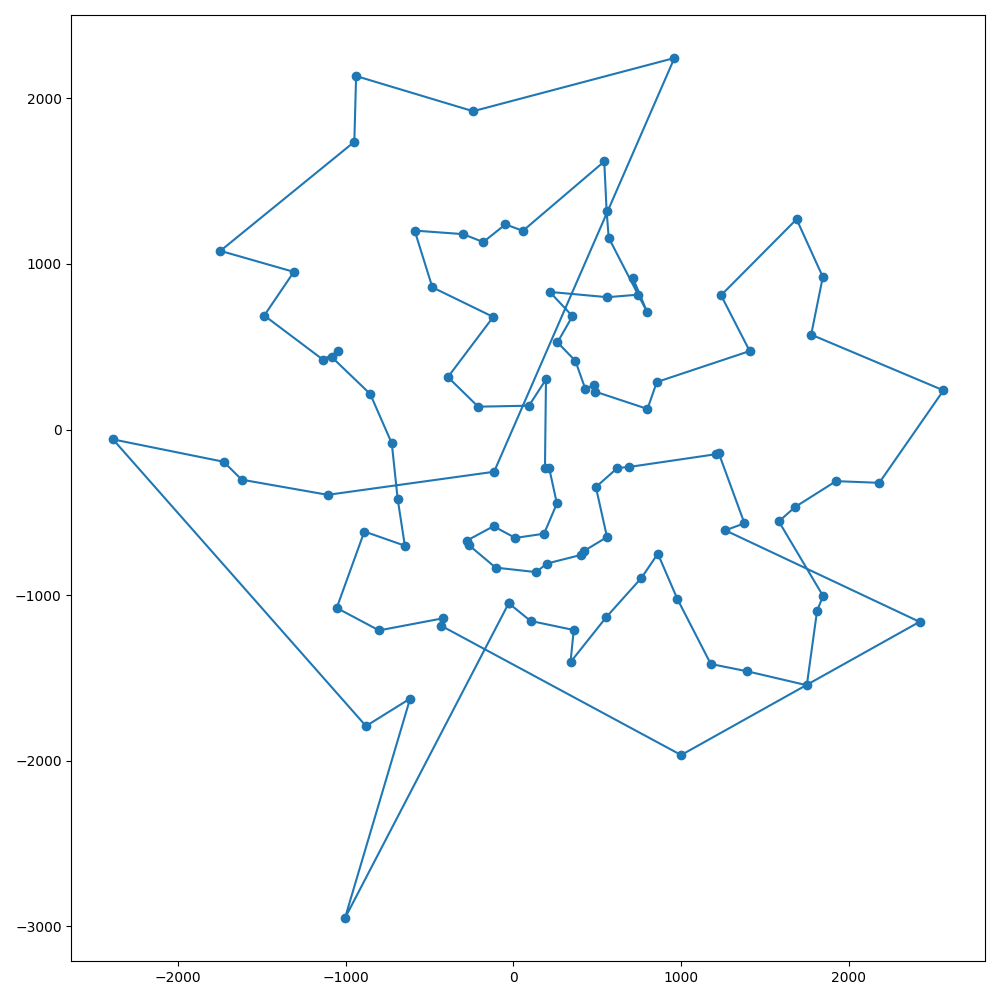
\includegraphics[width=6cm]{lab4/img/greedy/greed_1_0.png}}
            \subfloat[]{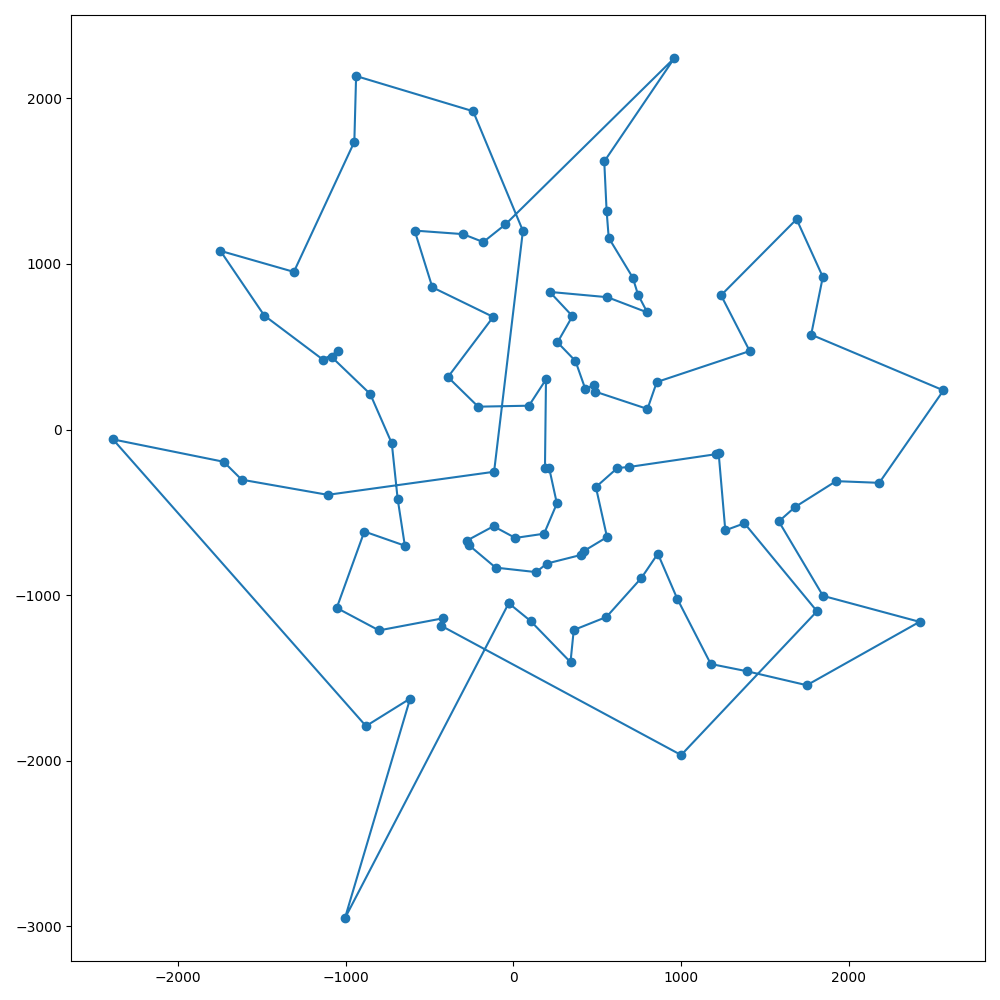
\includegraphics[width=6cm]{lab4/img/greedy/greed_1_1.png}}
            \subfloat[]{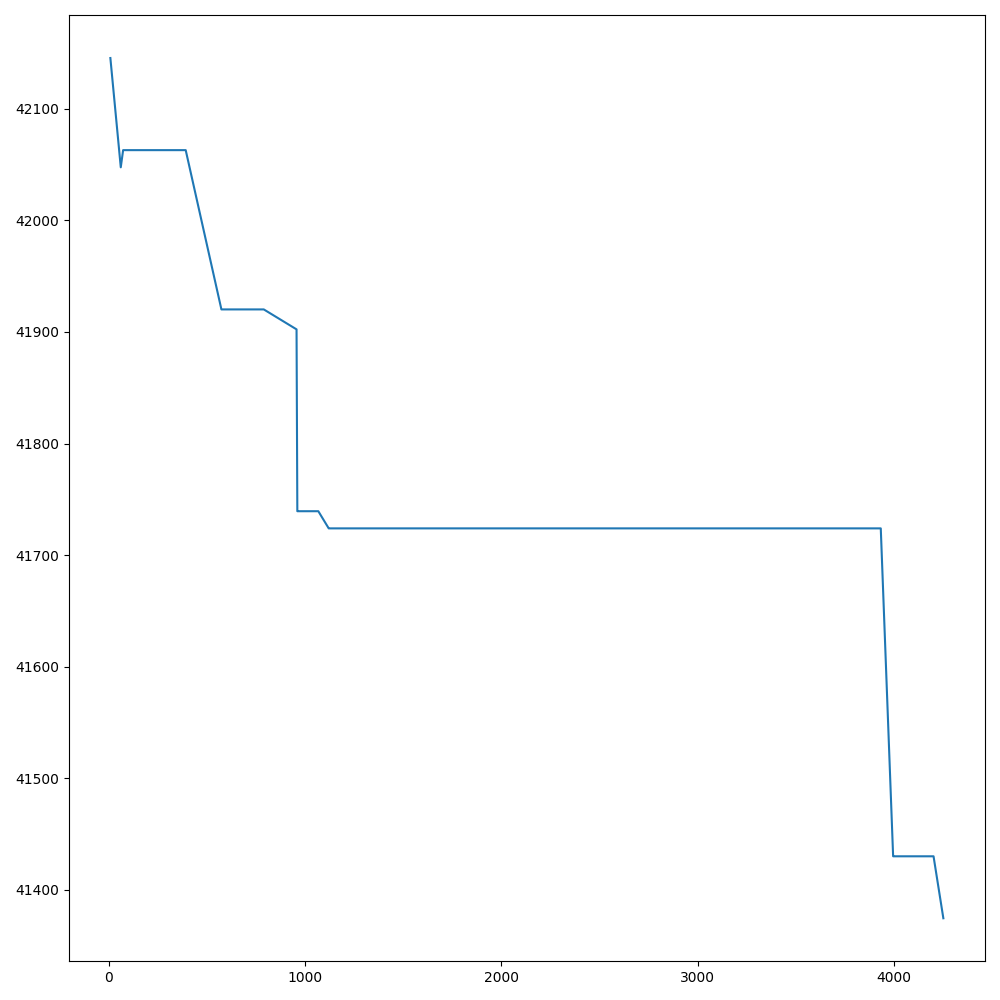
\includegraphics[width=6cm]{lab4/img/greedy/greed_1_2.png}}
            \caption{Rozkład normalny, $100$ punktów, temperatura $20$, optymalizacja trasy $3.6\%$}
        \end{figure}\\

        \begin{figure}[h!]
            \centering
            \subfloat[]{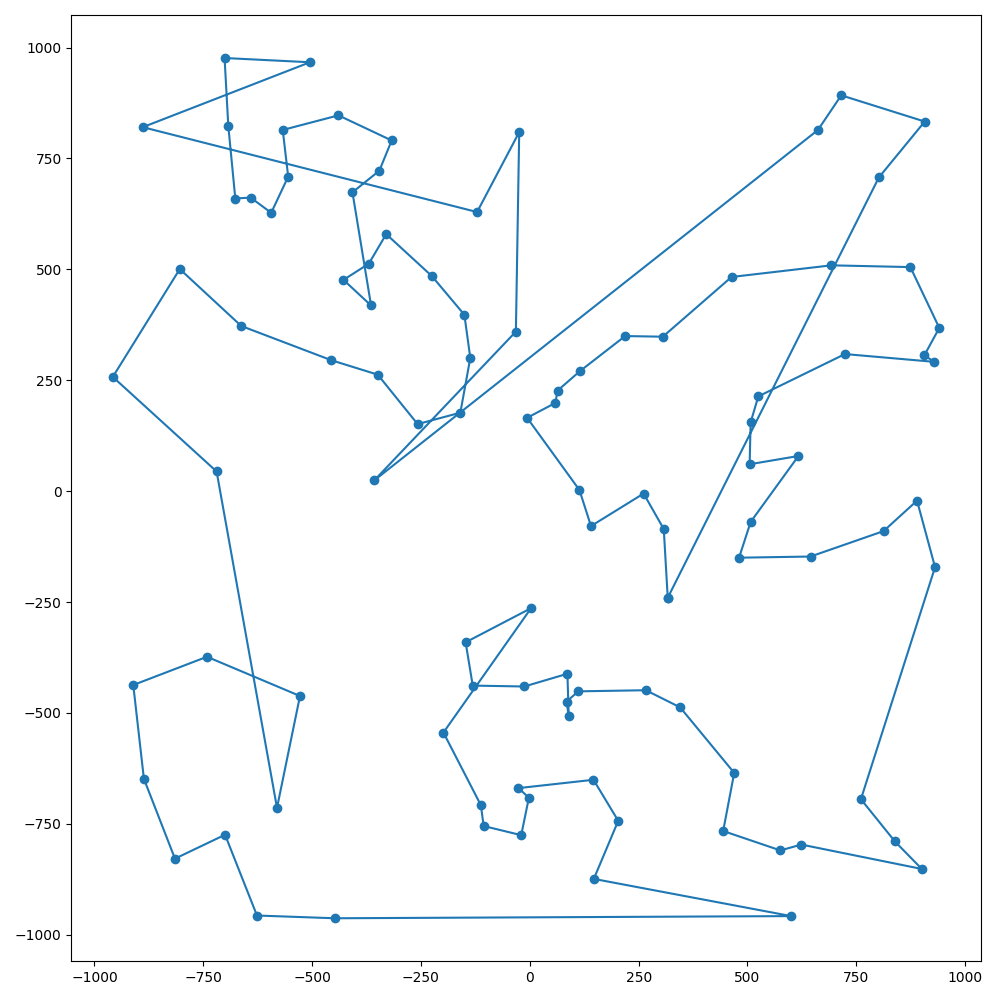
\includegraphics[width=6cm]{lab4/img/greedy/greed_2_0.png}}
            \subfloat[]{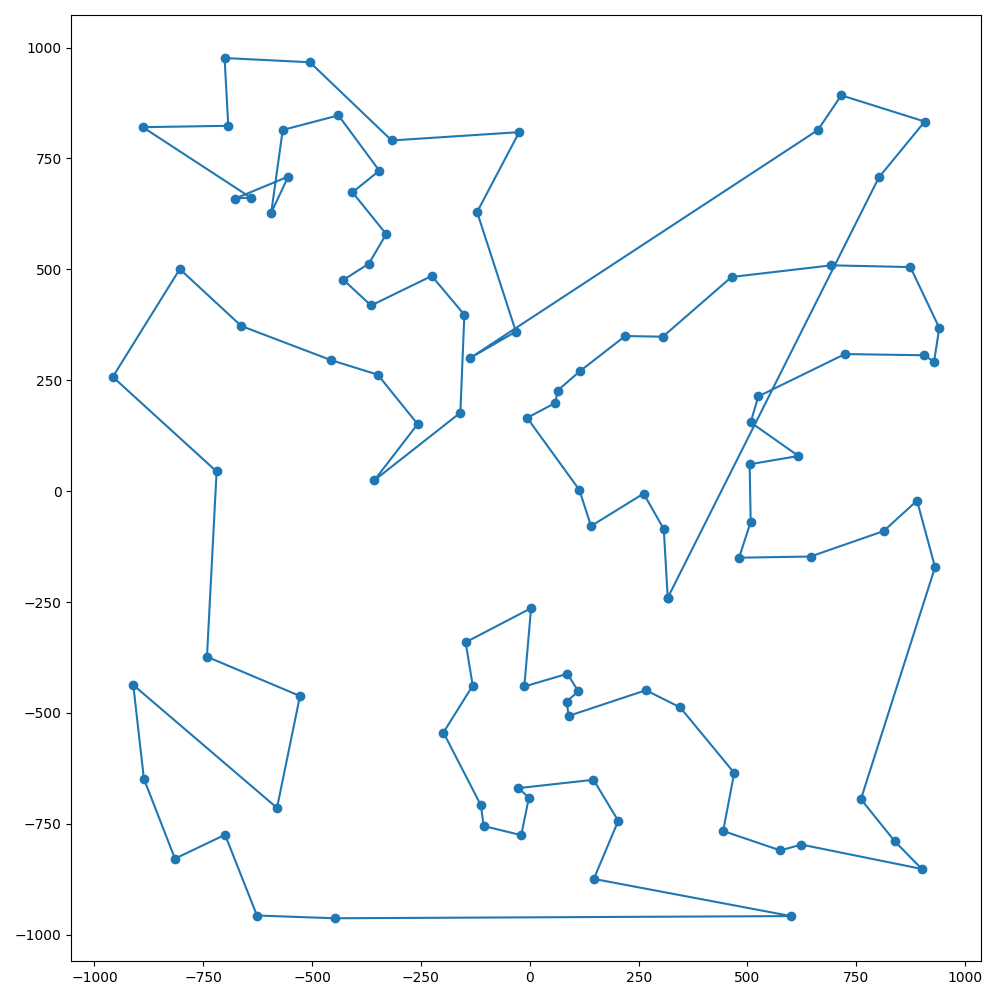
\includegraphics[width=6cm]{lab4/img/greedy/greed_2_1.png}}
            \subfloat[]{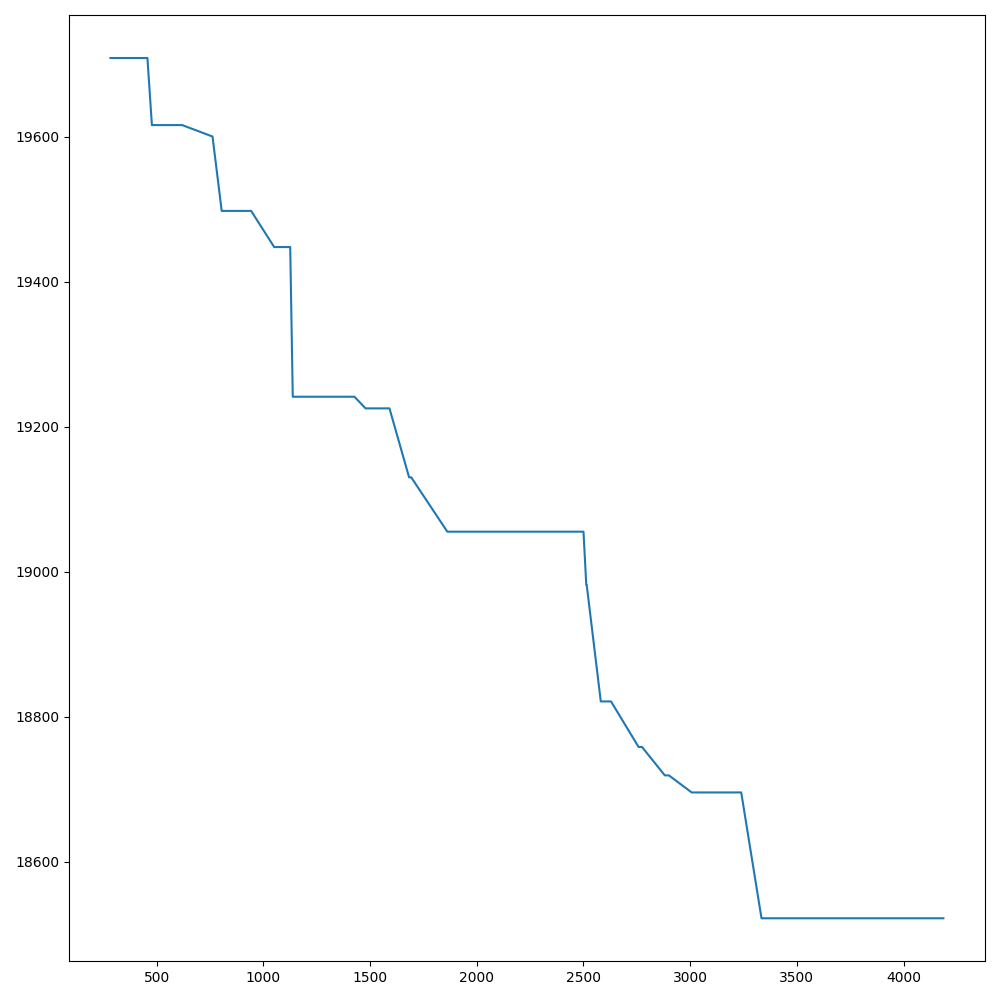
\includegraphics[width=6cm]{lab4/img/greedy/greed_2_2.png}}
            \caption{Rozkład normalny, $100$ punktów, temperatura $20$, optymalizacja trasy $6.1\%$}
        \end{figure}\\
        
    \clearpage
    \section{Minimalizacja funkcji energii dla obrazu binarnego}
        Następnie przygotowałem program generujący losowy, kwadratowy, obraz binarny o zadanym rozmiarze i gęstości czarnych punktów.
        Przygotowałem różne sąsiedztwa punktu, wyznaczające 4; 8; 16; 16+8 sąsiednich punktów w sposób przedstawiony w poniższej tabeli. 
        \begin{center}
            \begin{table}[ht]
                \centering
                \begin{tabular}{|c|c|c|c|c|}
                    \hline
                    16 & 16 & 16 & 16 & 16 \\
                    \hline
                    16 & 8 & 8; 4 & 8 & 16\\
                    \hline
                    16 & 8; 4 &  & 8; 4 & 16\\
                    \hline
                    16 & 8 & 8; 4 & 8 & 16\\
                    \hline
                    16 & 16 & 16 & 16 & 16\\
                    \hline 
                \end{tabular}
                \caption{Graficzna reprezentacja sąsiedztwa.}
                \label{tab:my_label}
            \end{table}
        \end{center}\\  
        \FloatBarrier
        Przygotowałem też różne funkcje energii punktu, opisane poniżej.
        Niech d będzie odległością punktu sąsiedniego od rozpatrywanego w funkcji energii. 
        \begin{itemize}
            \item dist - Jeśli punkt sąsiedni ma tą samą wartość co rozpatrywany, zwraca -d dla punktów o odległości większej niż $\sqrt{2}$, d dla punktów bliższych. W przeciwnym przypadku 0.
            \item pushpull - Zwraca d jeśli punkt sąsiedni ma tą samą wartość co rozpatrywany, -d w przeciwnym wypadku. 
            \item diff - Zwraca -d jeśli punkt sąsiedni ma różną od rozpatrywanego wartość, 0 w przeciwnym przypadku. 
            \item on - Zwraca -d jeśli zarówno punkt sąsiedni jak i rozpatrywany ma wartość 1, 0 w przeciwnym przypadku. 
        \end{itemize}
        Tak przygotowany program testowałem z parametrami: Obraz rozmiaru 64x64, ilość kroków algorytmu wyżarzania $10^{12}$, temperatura 80, współczynnik $\alpha = 0.9995$. Następny obraz wyznaczany jest poprzez losową zamianę dwóch dowolnych punktów. Funkcja kosztu obrazu zoptymalizowana jest, by w następnym kroku liczyć wartości tylko w tych polach, które uległy zmianie.\\
        Przykładowe wyniki działania programu: 
        \begin{figure}[h!]
            \centering
            \subfloat[Przed]{
\includegraphics[width=6cm]{lab4/img/bin_img/z1_0.png}}
            \subfloat[Po]{
\includegraphics[width=6cm]{lab4/img/bin_img/z1_1.png}}
            \subfloat[Funkcja kosztu]{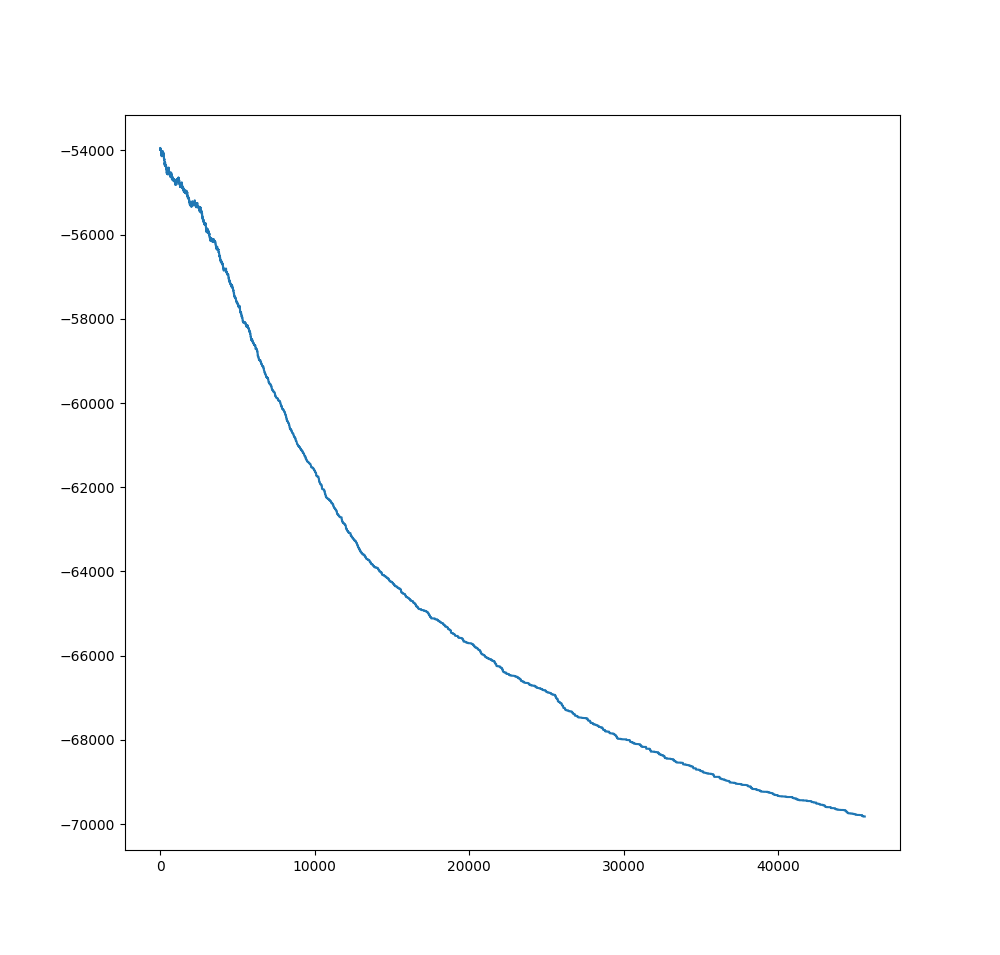
\includegraphics[width=6cm]{lab4/img/bin_img/z1_2.png}}
            \caption{Sąsiedztwo: 16+8, funkcja energii: dist.}
        \end{figure}\\
        \begin{figure}[h!]
            \centering
            \subfloat[Przed]{
\includegraphics[width=6cm]{lab4/img/bin_img/z2_0.png}}
            \subfloat[Po]{
\includegraphics[width=6cm]{lab4/img/bin_img/z2_1.png}}
            \subfloat[Funkcja kosztu]{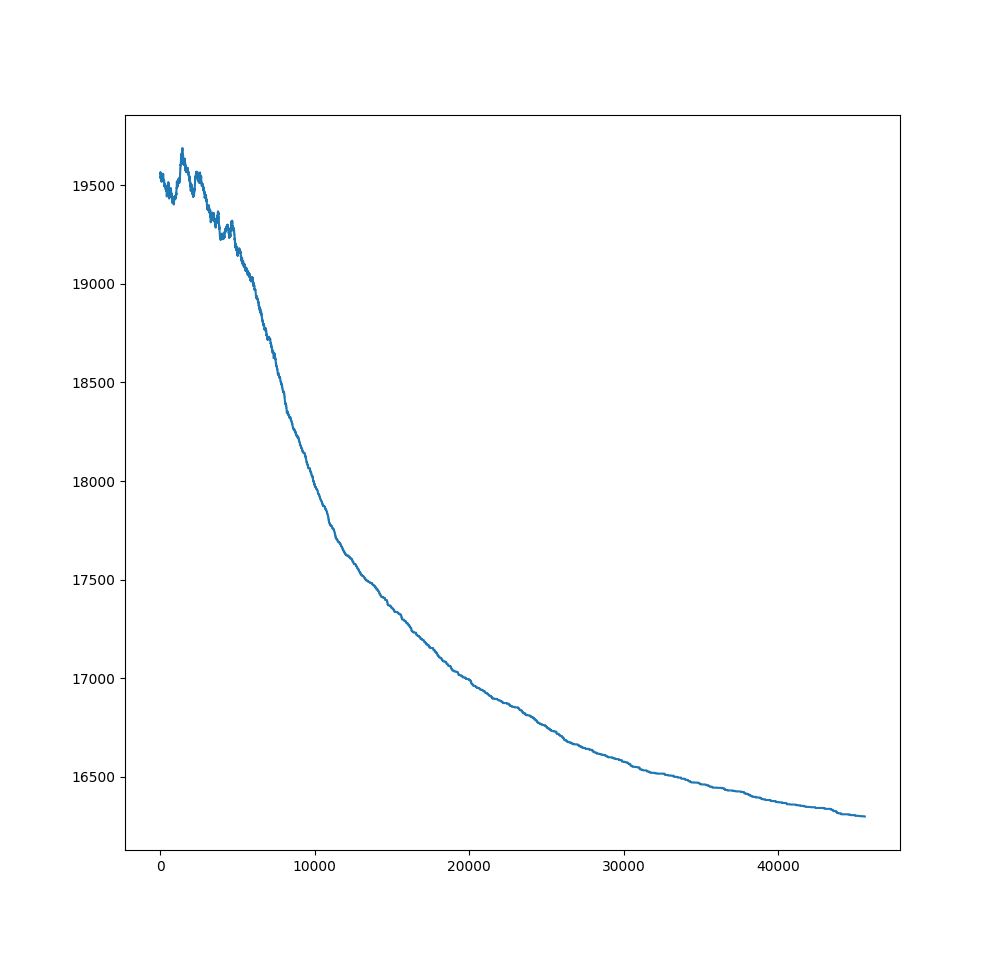
\includegraphics[width=6cm]{lab4/img/bin_img/z2_2.png}}
            \caption{Sąsiedztwo: 8, funkcja energii: dist.}
        \end{figure}\\
        \begin{figure}[h!]
            \centering
            \subfloat[Przed]{
\includegraphics[width=6cm]{lab4/img/bin_img/z3_0.png}}
            \subfloat[Po]{
\includegraphics[width=6cm]{lab4/img/bin_img/z3_1.png}}
            \subfloat[Funkcja kosztu]{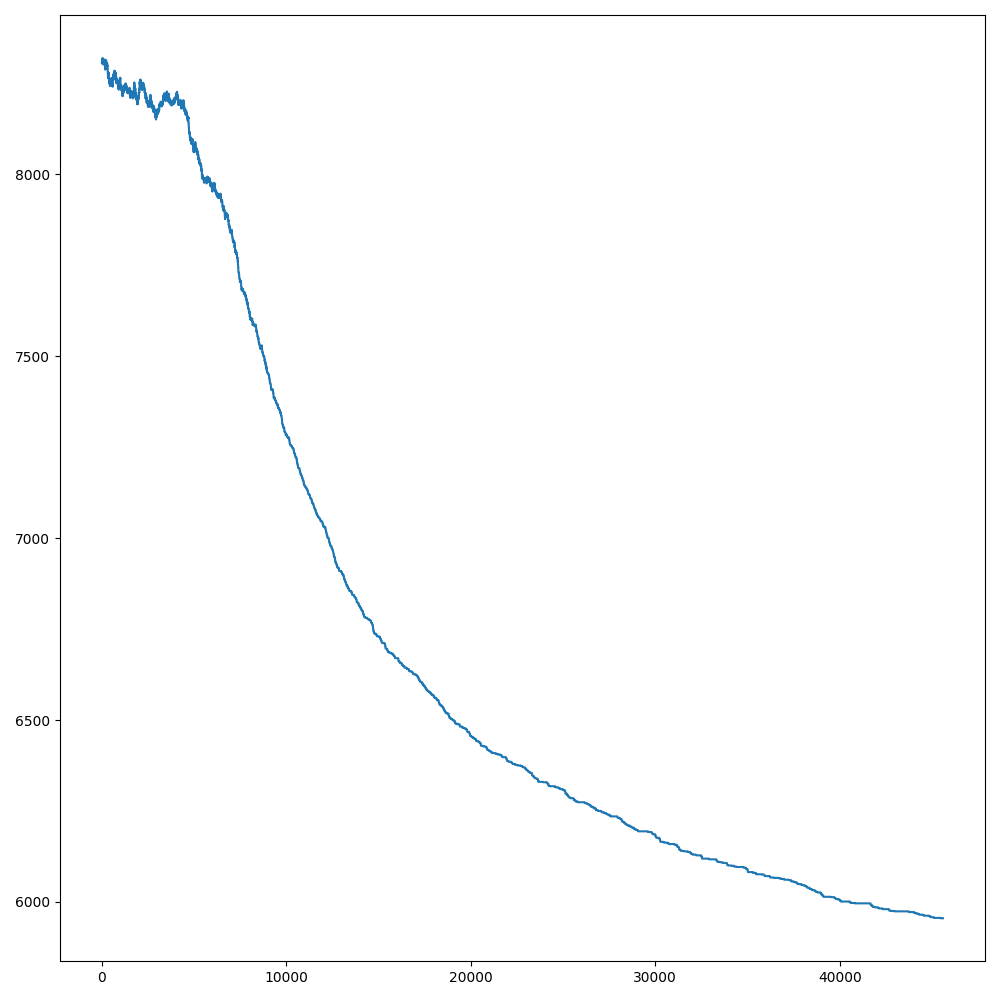
\includegraphics[width=6cm]{lab4/img/bin_img/z3_2.png}}
            \caption{Sąsiedztwo: 4, funkcja energii: dist.}
        \end{figure}\\
        \begin{figure}[h!]
            \centering
            \subfloat[Przed]{
\includegraphics[width=6cm]{lab4/img/bin_img/z4_0.png}}
            \subfloat[Po]{
\includegraphics[width=6cm]{lab4/img/bin_img/z4_1.png}}
            \subfloat[Funkcja kosztu]{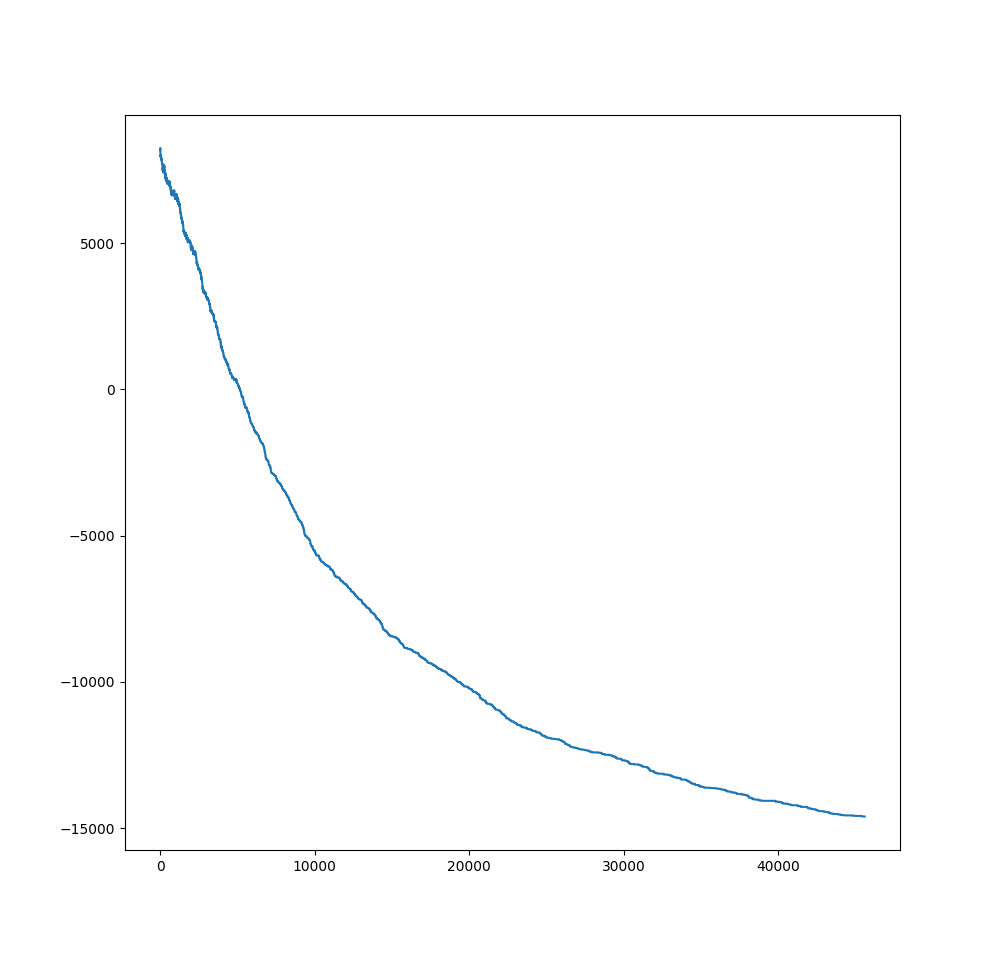
\includegraphics[width=6cm]{lab4/img/bin_img/z4_2.png}}
            \caption{Sąsiedztwo: 16+8, funkcja energii: pushpull.}
        \end{figure}\\
        \begin{figure}[h!]
            \centering
            \subfloat[Przed]{
\includegraphics[width=6cm]{lab4/img/bin_img/z5_0.png}}
            \subfloat[Po]{
\includegraphics[width=6cm]{lab4/img/bin_img/z5_1.png}}
            \subfloat[Funkcja kosztu]{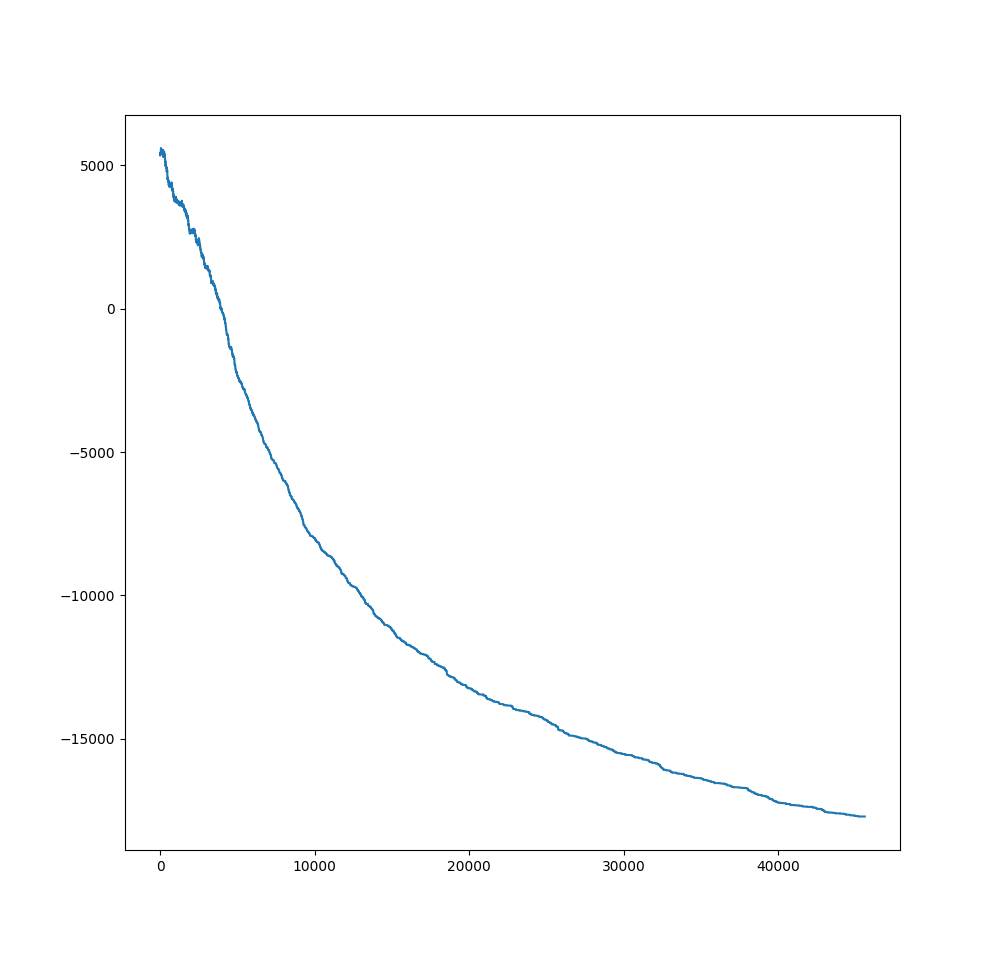
\includegraphics[width=6cm]{lab4/img/bin_img/z5_2.png}}
            \caption{Sąsiedztwo: 16, funkcja energii: pushpull.}
        \end{figure}\\
        \begin{figure}[h!]
            \centering
            \subfloat[Przed]{
\includegraphics[width=6cm]{lab4/img/bin_img/z6_0.png}}
            \subfloat[Po]{
\includegraphics[width=6cm]{lab4/img/bin_img/z6_1.png}}
            \subfloat[Funkcja kosztu]{\includegraphics[width=6cm]{lab4/img/bin_img/z6_2.png}}
            \caption{Sąsiedztwo: 8, funkcja energii: pushpull.}
        \end{figure}\\
        \begin{figure}[h!]
            \centering
            \subfloat[Przed]{\includegraphics[width=6cm]{lab4/img/bin_img/z7_0.png}}
            \subfloat[Po]{\includegraphics[width=6cm]{lab4/img/bin_img/z7_1.png}}
            \subfloat[Funkcja kosztu]{\includegraphics[width=6cm]{lab4/img/bin_img/z7_2.png}}
            \caption{Sąsiedztwo: 16+8, funkcja energii: diff.}
        \end{figure}\\
        \begin{figure}[h!]
            \centering
            \subfloat[Przed]{\includegraphics[width=6cm]{lab4/img/bin_img/z8_0.png}}
            \subfloat[Po]{\includegraphics[width=6cm]{lab4/img/bin_img/z8_1.png}}
            \subfloat[Funkcja kosztu]{\includegraphics[width=6cm]{lab4/img/bin_img/z8_2.png}}
            \caption{Sąsiedztwo: 16, funkcja energii: diff.}
        \end{figure}\\
        \begin{figure}[h!]
            \centering
            \subfloat[Przed]{\includegraphics[width=6cm]{lab4/img/bin_img/z9_0.png}}
            \subfloat[Po]{\includegraphics[width=6cm]{lab4/img/bin_img/z9_1.png}}
            \subfloat[Funkcja kosztu]{\includegraphics[width=6cm]{lab4/img/bin_img/z9_2.png}}
            \caption{Sąsiedztwo: 8, funkcja energii: diff.}
        \end{figure}\\
        % \begin{figure}[h!]
        %     \centering
        %     \subfloat[Przed]{\includegraphics[width=6cm]{lab4/img/bin_img/}}
        %     \subfloat[Po]{\includegraphics[width=6cm]{lab4/img/bin_img/}}
        %     \subfloat[Funkcja kosztu]{\includegraphics[width=6cm]{lab4/img/bin_img/}}
        %     \caption{Sąsiedztwo: , funkcja energii: .}
        % \end{figure}\\

    \clearpage
    \section{Sudoku}
        Przygotowałem program poszukujący rozwiązania dla planszy sudoku metodą symulowanego wyżarzania. Jako funkcję kosztu przyjąłem sumę powtórzeń cyfr w wierszach i kolumnach planszy, oraz w blokach o rozmiarze 3x3. Przy wczytywaniu planszy z pliku tekstowego, oznaczam puste pola jako modyfikowalne. Uzupełniam je także brakującymi w całej planszy cyframi. Stan następny wyznaczam zamieniając dowolne dwie modyfikowalne pozycje. \\
        Program testowałem z użyciem parametrów: temperatura 400, współczynnik $alpha = 0.9995$, liczba kroków $10^{12}$.\\
        Przykłady działania programu. 
        \begin{figure}[h!]
            \centering
            \subfloat[]{\includegraphics[width=6cm]{lab4/img/sudoku/s1_0.png}}
            \subfloat[]{\includegraphics[width=6cm]{lab4/img/sudoku/s1_1.png}}
            \caption{Przykład 1.}
        \end{figure}\\
        \begin{figure}[h!]
            \centering
            \subfloat[]{\includegraphics[width=6cm]{lab4/img/sudoku/s2_0.png}}
            \subfloat[]{\includegraphics[width=6cm]{lab4/img/sudoku/s2_1.png}}
            \caption{Przykład 2.}
        \end{figure}\\
        \begin{figure}[h!]
            \centering
            \subfloat[]{\includegraphics[width=6cm]{lab4/img/sudoku/s1_0.png}}
            \subfloat[]{\includegraphics[width=6cm]{lab4/img/sudoku/s1_1.png}}
            \caption{Przykład 3.}
        \end{figure}\\
        
        
        \FloatBarrier 
        Zauważyłem, że program nie zwraca poprawnego rozwiązania planszy sudoku w każdym przypadku. Koszt końcowej planszy waha się także pomiędzy uruchomieniami programu. 


\end{document}